% Opcje klasy 'iithesis' opisane sa w komentarzach w pliku klasy. Za ich pomoca
% ustawia sie przede wszystkim jezyk oraz rodzaj (lic/inz/mgr) pracy.
\documentclass[shortabstract, lic, english]{iithesis}

\usepackage[utf8]{inputenc}

%%%%% DANE DO STRONY TYTUŁOWEJ
% Niezaleznie od jezyka pracy wybranego w opcjach klasy, tytuł i streszczenie
% pracy nalezy podac zarowno w jezyku polskim, jak i angielskim.
% Pamietaj o madrym (zgodnym z logicznym rozbiorem zdania oraz estetyka) recznym
% złamaniu wierszy w temacie pracy, zwłaszcza tego w jezyku pracy. Uzyj do tego
% polecenia \fmlinebreak.
\englishtitle   {Experimental Comparison of \fmlinebreak (2,1)-Distance~Oracles}
\polishtitle    {Eksperymentalne porównanie \fmlinebreak wyroczni~odległości~(2,1)}
\englishabstract{
    Let $G~=~(V,~E)$ be an undirected unweighted graph with $|V|~=~n$ vertices and $|E|~=~m$ edges.
Let $\delta(u,~v)$ denote the distance between vertices $u,~v~\in~V$.
An $(\alpha,\beta)-approximate$ distance oracle for $G$ is a data structure that supports the following distance queries between pair of vertices in $G$:
Given two vertices $u,~v$ it can in constant time compute a distance estimate $\hat{\delta}(u,~v)$ that satisfies 
$$\delta(u,~v)~\leq~\hat{\delta}(u,~v)~\leq~\alpha\delta(u, v)~+~\beta$$
What is remarkable in this structure is that it can take significantly less than quadratic space,
but still answer distance queries in constant time,
despite quadratic space structure required to retrieve exact distances.
The $(3,0)$ distance oracle is the most precise oracle that have $\beta=0$ and takes only $O(n^{2-\epsilon})$ memory $-$ $O(n^{3/2})$ to be exact.
By using the additive error $-$~$\beta>0$ we are able to decrease $\alpha$ to $2$ preserving the $O(n^{2-\epsilon})$ memory $-$ $(2,1)$ distance oracle takes only $O(n^{5/3})$ memory.
Unfortunately the Oracle with additive error no longer works on weighted graphs, only on unweighted.
In this paper we will compare $(2,1)$ distance oracles on different graph sets, looking at their memory use, query time and average error.
We will also compare the preprocessing time.
}
\polishabstract {
    Niech $G~=~(V,~E)$ będzie nieskierowanym, nieważonym grafem, gdzie $n~=~|V|$ jest liczbą wierzchołków, a $m~=~|E|$ liczbą krawędzi.
Oznaczmy jako $\delta(u,~v)$ odległość pomiędzy wierzchołkami $u,~v~\in~V$.
Wyrocznią odległości $(\alpha,\beta)$-przybliżoną grafu $G$, gdzie $\alpha~\geq 1,~\beta~\geq~0$ nazwiemy strukturę danych, która umożliwia następujące zapytania o odległości pomiędzy parami wierzchołków $G$:
Mając wierzchołki $u,~v$ możemy w stałym czasie policzyć przybliżoną odległość $\hat{\delta}(u,~v)$, która spełnia 
$$\delta(u,~v)~\leq~\hat{\delta}(u,~v)~\leq~\alpha\delta(u, v)~+~\beta$$
To co jest w tej strukturze niezwykłe to to, że może ona zajmować znacznie mniej niż kwadratowo wiele pamięci ale odpowiedzi na zapytania, których wszystkich możliwych jest kwadratowo wiele, pozostają w czasie stałym.
\newline 
Wyrocznia odległości~$(3,0)$ jest najdokładniejszą wyrocznią, która ma $\beta=0$ i dodatkowo zajmuje tylko $O(n^{2-\epsilon})$ pamięci $-$ dokładniej $O(n^{3/2})$.
Jednak używając błędu addytywnego $-$~$\beta>0$ jesteśmy w stanie zmniejszyć $\alpha$ do $2$ zachowując pamięć $O(n^{2-\epsilon})$ $-$ wyrocznia odległości~$(2,1)$ zajmuje jedynie $O(n^{5/3})$ pamięci.
Niestety wyrocznia z błędem addytywnym nie działa na grafy ważone, jedynie na nieważone.
W poniższej pracy porównamy na różnych zestawach grafów kilka wyroczni odległości (2,1) pod względem ich zajmowanej pamięci, szybkości działania i średniego błędu. Porównamy również czas jaki zajmuje stworzenie wyroczni.

}

% w pracach wielu autorow nazwiska mozna oddzielic poleceniem \and
\author         {Artur Błaszkiewicz}
% w przypadku kilku promotorow, lub koniecznosci podania ich afiliacji, linie
% w ponizszym poleceniu mozna złamać poleceniem \fmlinebreak
\advisor        {dr Paweł Gawrychowski}
%\date          {}                     % Data złozenia pracy
% Dane do oswiadczenia o autorskim wykonaniu
%\transcriptnum {}                     % Numer indeksu
%\advisorgen    {dr. Jana Kowalskiego} % Nazwisko promotora w dopełniaczu
%%%%%

%%%%% WŁASNE DODATKOWE PAKIETY
%
% \usepackage{graphicx,listings,amsmath,amssymb,amsthm,amsfonts,tikz}
%
%%%%% WŁASNE DEFINICJE I POLECENIA
%
%\theoremstyle{definition} \newtheorem{definition}{Definition}[chapter]
%\theoremstyle{remark} \newtheorem{remark}[definition]{Observation}
%\theoremstyle{plain} \newtheorem{theorem}[definition]{Theorem}
%\theoremstyle{plain} \newtheorem{lemma}[definition]{Lemma}
%\renewcommand \qedsymbol {\ensuremath{\square}}
% ...
%%%%%

\usepackage{amsthm, amssymb}
\theoremstyle{definition} \newtheorem{definition}{Definition}[chapter]
\theoremstyle{remark} \newtheorem{remark}[definition]{Observation}
\theoremstyle{plain} \newtheorem{theorem}[definition]{Theorem}
\theoremstyle{plain} \newtheorem{lemma}[definition]{Lemma}
\renewcommand \qedsymbol {\ensuremath{\square}}

\theoremstyle{plain} \newtheorem{conjecture}[definition]{Conjecture}

\usepackage{mathtools}
\DeclarePairedDelimiter{\ceil}{\lceil}{\rceil}
\DeclarePairedDelimiter{\floor}{\lfloor}{\rfloor}
\usepackage{algorithm}
\usepackage{algpseudocode}
\usepackage{multirow}
\usepackage{graphicx, subcaption}
\graphicspath{ {./images/} }


\begin{document}

%%%%% POCZĄTEK ZASADNICZEGO TEKSTU PRACY

\chapter{Introduction}

In chapter \ref{theoreticalLimitations} we will discuss why $(3,0)$ and $(2,1)$ distance oracles
have minimum possible error allowing for subquadratic space structure.
Next, in chapter \ref{30DistanceOracle} we will present the basic $(3,0)$ distance oracle by Thorup and Zwick \cite{a0OraclesBasic}
chapter \ref{21DistanceOracle} will be dedicated to how the $(3,0)$ multiplicative error barrier was breached by adding the additive error $-$
$(2,1)$ distance oracle, sacrificing weighted graphs and some memory in the process.
The next two chapters will be dedicated to the different variations of the $(2,1)$ distance oracle,
in the chapter \ref{21TheoreticalComparison} we will discuss the theoretical differences,
while in the chapter \ref{21PracticalComparison} we will show the results of the tests on different graph sets.

The main contribution of this paper is modifying the oracles \cite{a0OraclesBasic} \cite{21OracleBasic} \cite{21OracleLessMemory} in a way that they are all more similar to each other,
expanding proofs, verifying claims and improving the bounds of a few steps basing on claims from future papers.
We also show how to adapt $(2,1)$ distance oracle to weighted graphs $(2,\text{max\_edge\_weight})$ distance oracle as claimed possible by \cite{21OracleSpannerNoPenalty}.
Finally the oracles were implemented for unweighted graphs and tested on random graphs with a particular density. We also constructed unweighted graph realizing log factors from algorithm $\mathbf{center}(G, s)$ of \cite{samplingTechnique},
making the bounds of \cite{21OracleBasic} tight for that particular oracle construction.

\begin{definition}
    Surplus $t$ estimate for $t>0$ is any estimate $\hat{\psi}$ of a value $\psi$ that satisfies $\psi \leq \hat{\psi} \leq \psi + t$
    It is also called the additive error estimate.
\end{definition}

\begin{definition}
    Stretch $t$ estimate for $t>1$ is any estimate $\hat{\psi}$ of a value $\psi$ that satisfies $\psi \leq \hat{\psi} \leq t\psi$.
    It is also called the multiplicative error estimate.
\end{definition}

\begin{definition}
    % It is also called Stretch $(\alpha, \beta)$ estimate
    $(\alpha, \beta)$-approximation for $\alpha \geq 1, \beta \geq 0$ is any estimate $\hat{\psi}$ of a value $\psi$ that satisfies $\psi \leq \hat{\psi} \leq \alpha\psi + \beta$.
    $(\alpha, \beta)$-approximation have additive and multiplicative errors combined, when $\alpha > 1, \beta > 0$.
\end{definition}
    Usually when $\beta > 0$ the graph is assumed to be unweighted or $\beta$ depends on the largest edge.

The $(\alpha,\beta)-approximate$ distance oracle or in short $(\alpha,\beta)$ distance oracle returns stretch $(\alpha,\beta)$ estimates.

\begin{definition}
    Single-Source Shortest Path or SSSP Problem consists of finding the distances between a given vertex $v$ and all other vertices in the graph. 
\end{definition}

\begin{definition}
    All-Pairs Shortest Path or APSP Problem consists of finding the distances between all pairs of vertices in the graph. 
\end{definition}

\begin{definition}
    All-Pairs $Approximate$ Shortest Path or APASP Problem consists of finding approximate distances between all pairs of vertices in the graph. 
\end{definition}

\chapter{Theoretical Limitations} \label{theoreticalLimitations}

\section{Space Lower Bound}
\begin{definition}
    A simple cycle is a path that have distinct edges and only the first and the last of its vertices are equal.
\end{definition}

\begin{definition} 
    The girth of the graph is the length of it's shortest simple cycle. 
\end{definition}

\begin{theorem} \label{lotsOfEdgesLittleGirth}
    A graph with at least $\frac{1}{2} * n^{1 + 1/k}$ edges 
    have girth not greater than $2k$
\end{theorem}


\begin{proof}
    We will prove the lemma for $k=2$. Full proof can be found in Alon $et~al.$~\cite{alon}.
    \newline
    Suppose that there exist graph $G$ with $\frac{1}{2} * n^{1 + 1/k}$ or more edges, that have girth at least $2k+1$.
    In other words $G$ does not have a simple cycle of length $2k$ or less.
    \newline
    The vertex $u$ have degree $deg(u)~=~a$ when number of edges incident to $u$ plus number of edges connecting $u$ with itself (loops) amounts to $a$
    \footnote{Every loop is also incident to its vertex}.
    \newline
    Let $nei_a(v)~=~\{u~\in~V~|~\delta(v,~u)~=~a\}$
    \newline
    For $2~\leq~i~\leq~k$ we show that
    $$|nei_{i}(v)| = \sum_{u \in nei_{i-1}(v)} (deg(u)-1)$$
    as
    \newline
    1. Every vertex $u$ from set $nei_{i-1}(v)$ have exactly one edge $(u, l)$
    such that $\delta(v, l)\leq i-1$
    \newline
    and 
    \newline
    2. There is no two distinct edges $(u, l),~(w, l)$ satisfying $u,w \in nei_{i-1}(v),$ $l\in~V$ 


    \begin{figure}[h]
    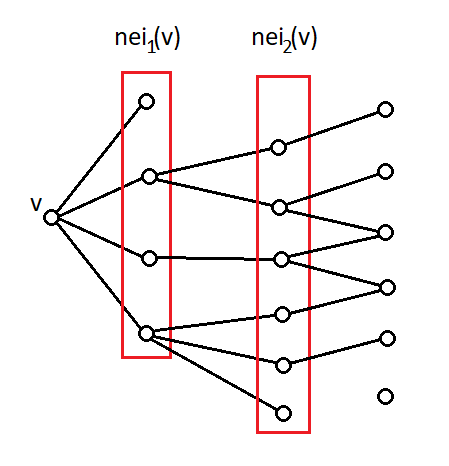
\includegraphics[width=8cm]{images/placeholder_neikv}
    \centering
    \caption{Placeholder for $|nei_{2}(v)|$}
    \end{figure}

    \newpage

    We note that $u\in nei_i(v) \iff v\in nei_i(u)$, so for $2~\leq~i~\leq~k$ we have:
    $$\sum_{v \in V}|nei_i(v)|~=
    ~\sum_{v \in V}\sum_{u \in nei_{i-1}(v)} (deg(u) - 1)~=$$
    $$=~\sum_{u \in V}\sum_{v \in nei_{i-1}(u)}(deg(u) - 1)$$
    $$=~\sum_{u \in V}((|nei_{i-1}(u)|)*(deg(u) - 1))$$
    For every $v~\in~V$ the following is true:
    \begin{equation}\label{allNeighboursCount}
    \sum_{i=0}^{k} |nei_i(v)|=|\{u~\in~V~|~\delta(v,~u)~\leq~k\}|~\leq~|V|~=~n
    \end{equation}
    However, if we look at the sum:
    $$\sum_{v \in V}\sum_{i=0}^{k} |nei_i(v)|~=
    ~\sum_{v \in V}(1 + |nei_1(v)| + \sum_{i=2}^{k} |nei_i(v)|)~=$$
    $$=~n+\sum_{v \in V}(|nei_1(v)|)+\sum_{v \in V}\sum_{i=2}^{k} |nei_i(v)|~=$$
    $$=~n+\sum_{v \in V}(deg(v))+\sum_{v \in V}\sum_{i=2}^{k}\sum_{u \in nei_{i-1}(v)} (deg(u) - 1)~=~~(\textnormal{for}~k=2)$$
    $$=~n+\sum_{v \in V}(deg(v))+\sum_{v \in V}\sum_{u \in nei_1(v)} (deg(u) -1)~=$$
    $$=~n+\sum_{v \in V}(deg(v))+\sum_{u \in V}((|nei_1(u)|)*(deg(u) -1))~=$$
    $$=~n+\sum_{v \in V}(deg(v))+\sum_{u \in V}((deg(u))*(deg(u) -1))~=$$
    $$=~n+\sum_{u \in V}((deg(u))*(deg(u)))~\geq~n+n*(avg~deg)^2~=$$
    $$=~n+n*(n^{1/2})^2~=~n*(n+1)~>~n^2$$

    where $avg~deg = \frac{2m}{n}$ is the average degree of a vertex.

    This contradicts \ref{allNeighboursCount}
\end{proof}

It is conjectured by Erd{\"o}s \cite{erdos1963} and others that the Theorem \ref{lotsOfEdgesLittleGirth} is tight.
Namely, it is conjectured that for any $k\geq1$, that there are graphs with
$\Omega(n^{1 + 1/k})$ edges and girth greater than $2k$. The conjecture is known to be true for $k=1,2,3,5$

\begin{remark}
For any graph of girth $2k+1$ it's bipartisan subgraphs have girth $2k+2$ or greater as simple cycles in bipartisan graphs have even length and subgraphs can't have smaller girth.
\end{remark}

Since graphs with girth greater than $1$ do not have loops, they have a bipartisan subgraph with at least half the edges, so
there are graphs with at least $\Omega(n^{1 + 1/k})$ edges and girth greater than $2k+1$.

\begin{lemma}
    An $(\alpha, \beta)$ distance oracle 
    must use at least $m$ bits of storage for girth $k > \alpha + \beta + 1$ graphs, where $m$ is a number of edges.
\end{lemma}
\begin{proof}
    Let $G$ be a girth $k > \alpha + \beta + 1$ graph with $n$ vertices and $m$ edges.
    Let $H$ be any subgraph of $G$ and $\delta_H(u,v)$ be a distance between vertices $u$, $v$ in $H$.
    
    Consider any edge $(u, v)$ from $G$.
    If $(u, v)$ is in $H$ then $\delta_H(u,v) = 1$, but otherwise $\delta_H(u,v) \geq k - 1$, since the girth of $H$ is not less than $k$.
    The oracle will report distance between $u$ and $v$ at most $1*\alpha + \beta$, if edge $(u,v)$ in $H$,
    but not less than $k-1$ otherwise. 
    
    Consequently, the generated structure must be different for subgraphs of $G$ with different edge sets.
    There is $2^m$ subgraphs of $G$ with different edge sets, so for at least one of them the generated oracle must take $m$ bits of space.
\end{proof}

\begin{remark}
    An $(\alpha, \beta)$ distance oracle must take at least $\Omega(n^{1+1/k})$ memory, where
    $k=\ceil{(\alpha + \beta + 1)/2}$, if the 1963 Erd{\"o}s girth conjecture is true.
\end{remark}

\begin{remark}
    This points to the space lower bound of $\Omega(n^{3/2})$ for $(3,0)$ and $(2,1)$ distance oracles.
    The bound for $(3, 0)$ distance oracle is tight up to $\Theta(k~log~n)$ due to Oracle by Thorup and Zwick \cite{a0OraclesBasic},
    described in this paper.
    Additionally any oracle with $\alpha + \beta < 3$ must take at least $\ceil{\frac{n*(n-1)}{4}}$ bits of storage for some graphs as there exists girth $4$ graph with that many edges.
\end{remark}

\begin{conjecture} \label{setIntersectionQueries} \cite{21OracleLessMemory}
    Consider a data structure that preprocesses sets $S_1, \ldots, S_n \subseteq [X]$, and answers queries of the form "does $S_i$ intersect $S_j$?".
    Let $X = \text{lg}^c n$ for a large enough constant $c$.
    If the query takes constant time, the space must be $\Omega(n^2 /$ poly log $ n)$.
\end{conjecture}

\begin{theorem} \label{alphaAbove2} \cite{21OracleLessMemory}
    A distance oracle for undirected, unweighted graphs with $m = O(n $ poly log $ n)$ edges, which can distinguish between distances of $2$ and $4$ in constant time
    requires $O(n^2 $ poly log $ n)$ space assuming conjecture \ref{setIntersectionQueries}
\end{theorem}

\begin{proof}
    Build a bipartite graph, with $n$ vertices on the left, numbered from $1$ to $n$ and $X$ on the right, numbered $1$ to $X$. The number of vertices
    is $n + X = O(n)$. Connect left vertex $i$ to the elements of $S_i$ on the right. The number of edges is no more than $nX = O(n * $ poly log $n)$.
    Two left vertices are at distance $2$ if the corresponding sets intersect, and distance at least $4$ otherwise.
    Thus, the distance oracle can solve set intersection queries.
\end{proof}

\begin{figure}[h]
    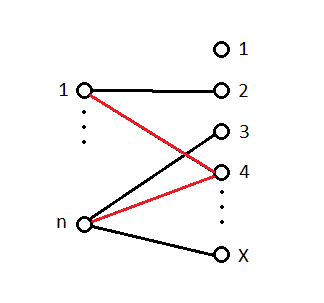
\includegraphics[width=8cm]{images/placeholder_setintersection}
    \centering
    \caption{Placeholder for Theorem \ref{alphaAbove2}}
\end{figure}

\begin{remark}
    For any graph we can insert $c-1$ vertices on each edge, splitting the edge into $c$ edges,
    so that each pair of the original vertices will have their distance multiplied by $c$, where $c$ is a positive integer.
    The number of vertices in the new graph will be $n + (c-1)m = O(n + m)$, number of edges will be $cm = O(m)$.
\end{remark}

In consequence any Oracle that can distinguish between distances $2c$ and $4c$ in constant time must use $\Omega(n'^2 /$ poly log $ n') = \Omega(n^2 /$ poly log $ n)$ space,
where $n = O(c * (n' * $ poly log $n'))$, so $n' = O(n/$ poly log $n)$.

An $(\alpha, \beta)$ distance oracle must take $O(n^2/ $ poly log $n)$ space if $\alpha < 2$, assuming conjecture \ref{setIntersectionQueries}

\section{Preprocessing Time Lower Bound}
% Maybe stretch less than $2$ and constant surplus?
The stretch $2$ or constant surplus distance oracle is smallest stretch oracle that possibly could calculate all distance estimates in less time than boolean matrix multiplication.
This is because any algorithm that computes all-pairs approximate distances with stretch less than $2$ (or surplus only)
could be used to compute boolean matrix multiplication \cite{matrixLowerBound}.

For directed graphs any constant stretch could be used to compute boolean matrix multiplication (also in \cite{matrixLowerBound})

$m^{5/3 - o(1)}$ time is required for a stretch $(2 + o(1))$ oracle based on 3-SUM conjecture\cite{3sumLowerBound}




\chapter{(3,0) Distance Oracle} \label{30DistanceOracle}
We present the slightly modified $(2k-1)-approximate$ distance oracle of Thorup and Zwick\cite{a0OraclesBasic}

\begin{theorem}
Let $G~=~(V,~E)$ be an undirected \underline{weighted} graph with non-negative weights and $|V|~=~n$ vertices and $|E|~=~m$ edges.
Let $\delta(u,v)$ denote the distance between vertices $u,v \in V$.
Let $k\geq1$ be an integer. The graph can be preprocessed in $O(nm + kn^2)$ expected time\footnote{
    by skipping All-Pairs Shortest Path preprocessing and preprocessing the graph directly it is possible to create the oracle in $O(n^2)$ expected time \cite{a0OraclesN2Time} or $O(mn^{1/k})$ deterministic time \cite{a0OraclesMN1KDeterministicTime}}
in order to obtain data structure of size $O(kn^{1+1/k})$ such that any distance approximation
$\hat{\delta}(u,v)$ satisfying $\delta(u,v)\leq \hat{\delta}(u,v)\leq (2k-1)\delta(u, v)$
can be retrieved in $O(k)$ time.
\end{theorem}

\begin{definition}
    A distance between sets $X, Y \subseteq V$ denoted $\delta(X,Y)$ is equal to the distance
    between closest vertices in those sets. 
    \newline
    More precisely 
    $\delta(X,Y) = \liminf\{\delta(u,v) ~|~ u\in X, v\in Y\}$ \newline
    A distance between vertex $v$ and set $X \subseteq V$ denoted $\delta(v,X)$ or $\delta(X,v)$
    is equal to $\delta(\{v\},X)$ or $\delta(X,\{v\})$ respectively.
\end{definition}

\begin{definition}
    A ball $B_X(v)$ for a given set $X \subseteq V$ and a vertex $v\in V$
    is a set of vertices $\{u \in V ~|~ \delta(v,u) < \delta(v, X)\}$. We call $\delta(v, X)$ a radius of ball $B_X(v)$
\end{definition}

\begin{definition}
    A cluster $C_X(v)$ is an inverse of ball 
    $u\in C_X(v) \iff v\in B_X(u)$ or in other words
    $C_X(v) = \{u \in V ~|~ \delta(u,v) < \delta(u, X)\}$
\end{definition}

\begin{figure}[h]
    \centering
    \begin{subfigure}[h]{0.495\textwidth}
        \centering
        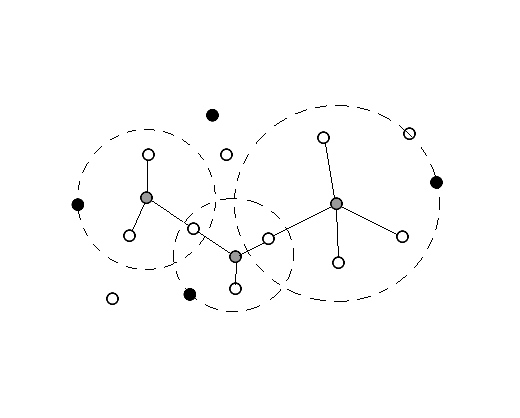
\includegraphics[height=5cm]{images/placeholder_ball}
        \caption{Placeholder for ball}
    \end{subfigure}
    \begin{subfigure}[h]{0.495\textwidth}
        \centering
        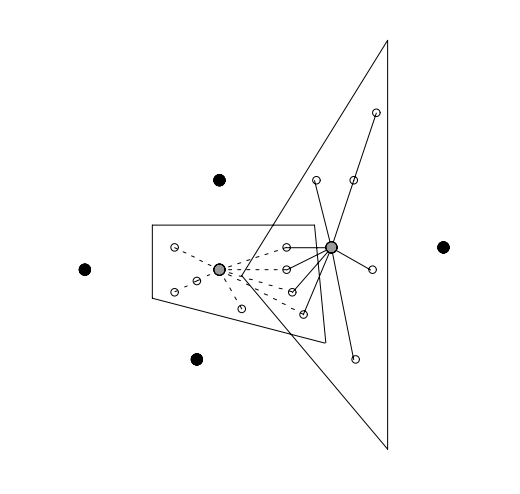
\includegraphics[height=5cm]{images/placeholder_cluster}
        \caption{Placeholder for cluster}
    \end{subfigure}
\end{figure}

Let $V = A_0 \supseteq A_1 \supseteq \ldots \supseteq A_k = \emptyset$ be a non increasing 
sequence of sets.

\begin{definition}
    A portal $p_{A_i}(v) \in A_i$ is a vertex that satisfies $\delta(v, p_{A_i}(v)) = \delta(v, A_i)$. Ties are broken arbitrarily. 
\end{definition}

\begin{definition}
    A bunch bun$(v) = \bigcup_{i=0}^{k-1}\{ u \in B_{A_{i+1}}(v) \cap A_i \}$
    \newline
    or more verbosely bun$(v) = \bigcup_{i=0}^{k-1}\{ u\in A_i \setminus A_{i+1} ~|~ \delta(v,u) < \delta(v, A_{i+1}) \}$
\end{definition}

\begin{definition}
    A clump clum$(v) = \bigcup_{i=0}^{k-1}\{ u \in C_{A_{i+1}}(v) \cap A_i \}$
    \newline
    or more verbosely clum$(v) = \bigcup_{i=0}^{k-1}\{ u\in A_i \setminus A_{i+1} ~|~ \delta(u,v) < \delta(u, A_{i+1}) \}$
\end{definition}

\begin{figure}[h]
    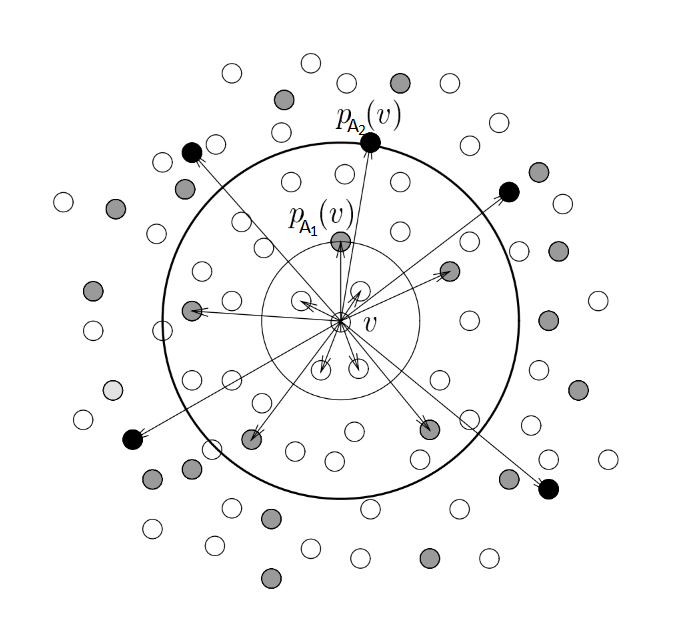
\includegraphics[width=10cm]{images/placeholder_bunch}
    \centering
    \caption{Placeholder for bunch}
\end{figure}

\noindent\fbox{
    \begin{minipage}{\textwidth -14.1pt}
    algorithm $\mathbf{basicprepro}_k(G)$

    calculate $\delta(u,v)$ for every $u,v \in V$

    $A_0 \leftarrow V ; A_k \leftarrow \emptyset$

    for $i \leftarrow 1$ to $k-1$

        ~~~~let $A_i$ be an uniform sample from $A_{i-1}$ of size $\ceil[\big]{n^{-1/k} * |A_{i-1}|}$

    for every $v \in V$

    ~~~~for $i \leftarrow 0$ to $k-1$

    ~~~~~~~~calculate $\delta(v, A_i)$ and $p_{A_i}(v)$

    % ~~~~$\delta(v, A_k) \leftarrow \infty$

    ~~~~calculate bun$(v)$

    return structure that for every $v, w \in V$, $0 \leq i \leq k-1$ can retrieve $p_{A_i}(v)$,

    ~~~~$\delta(v, u)$ for $u \in $ bun$(v)$ and can determine if $w \in $ bun$(v)$, all in constant time

    \end{minipage}
}

\noindent\fbox{
    \begin{minipage}{\textwidth -14.1pt}
    algorithm $\mathbf{basicdist}_k(u, v)$

    $w \leftarrow p_0(u) ; i \leftarrow 0$

    while $w \notin $ bun$(v)$

    ~~~~$i \leftarrow i+1$

    ~~~~$(u, v) \leftarrow (v, u)$

    ~~~~$w \leftarrow p_{A_i}(u)$

    return $\delta(u, w) + \delta(w, v)$

    \end{minipage}
}

As $n^{-1/k} > 0$ the sample size is greater than $0$, so $A_{i} \neq \emptyset$, for $0 \leq i < k$.

\section{Correctness}

The algorithm $\mathbf{basicdist}_k(u, v)$ always terminates in at most $k-1$ steps,
since $p_{k-1}(u) \in A_{k-1} \subseteq $ bun$(v)$ for every $u,v \in V$.
This means query time $O(k)$.

\begin{lemma}
$\delta(u, p_{A_i}(u))$ is at most $i*\delta(u,v)$
for as long as the $\mathbf{basicdist}_k(u, v)$ did not terminate in $i-1$ steps.
\end{lemma}
\begin{proof} 
The proof is by induction:
\newline
If the program terminates immediately then $\delta(u, p_0(u)) = \delta(u, u) = 0$.
\newline
If the program did not terminate in $i-1$ steps then 
\newline
$p_{i-1}(v) \notin $ bun$(u)$, so
$\delta(u, p_{i-1}(v)) \geq \delta(u, A_{i}) = \delta(u, p_{A_i}(u))$ and
\newline
$\delta(p_{i-1}(v), v) \leq (i-1)\delta(u, v)$, this combined gives
\newline
$\delta(u, p_{A_i}(u)) \leq \delta(u, p_{i-1}(v)) \leq \delta(p_{i-1}(v), v) + \delta(v, u) \leq i*\delta(u, v)$
\end{proof}

The distance returned by $\mathbf{basicdist}_k(u, v)$ is at most $(2k - 1)\delta(u,v)$ as
with the triangle inequality we have \newline
$\delta(u,p_{A_i}(u)) + \delta( p_{A_i}(u), v) \leq 2*\delta(u,  p_{A_i}(u)) + \delta(u,v) = (2i + 1)\delta(u,v) \leq (2k - 1)\delta(u,v)$


\section{Size of the Structure}

For each vertex $v \in V$ we store:
\begin{itemize}
    \item $p_{A_i}(v)$ for $i=0 \ldots k-1$ and its corresponding distance 
    $\delta(v, p_{A_i}(v)) = \delta(v, A_i)$
    \item the hash table for the bunch bun$(v)$ holding $\delta(v, u)$ for every $u \in $ bun$(v)$
    (the~hash~table is also able to determine whatever $u \in $ bun$(v)$ )
\end{itemize}

In order to store balls and distances in constant memory per entry and constant retrieve time we will use hash tables.
They can be computed in linear expected time\cite{2LevelHashTable} or
they can be computed deterministically is $O(s $ log $ s $ log $ n)$ time.\cite{hashTableDerandomization}, where $s$ in number of entries to be stored.

The total size of the data structure is $O(kn + \sum_{v \in V}|$bun$(v)|)$

\begin{lemma} \label{ballSize}
    Let $X \subseteq V$, $S$ be an uniform sample from $X$ of size $\ceil[\big]{p * |X|}$.
    Then for $v \in V$ the expected size of $B_{S}(v) \cap X$ is less than $1/p$.
\end{lemma}

\begin{proof}
    For we show that expected size of $B_{S}(v) \cap X$ is
    $stochastically$ $dominated$ by a random variable with parameter $p$.
    Let $w_1, w_2 \ldots w_l$ be the elements of $X$ arranged in any non-decreasing order of distance from $v$.
    If $w_j \in S$ then $w_j, w_{j+1}, \ldots , w_l \notin B_{S}(v)$
    as those elements are not closer to $v$ than $S$.

    If we look at Pr$[w_j \in S] \geq p$ we see that 
    $$\text{Pr}[w_j \in B_{S}(v)] \leq
    \text{Pr}[\{w_1, w_2, \ldots, w_j\} \cap S = \emptyset] \leq (1 - p)^j$$
    
    $$\mathbf{E}[B_{S}(v) \cap X] = \sum_{j=1}^{l} \text{Pr}[w_j \in B_{S}(v)] \leq \sum_{j=1}^{l}(1-p)^j < p^{-1}$$
\end{proof}

\begin{theorem} \label{ballSizeStrong}
    Let $X \subseteq V$, $S$ be an uniform sample from $X$ of size $q*\ceil[\big]{p * |X|}$, where $q$ is an positive integer.
    Then for $v \in V$ the expected value of $|B_{S}(v) \cap X|^q$ is less than $1/p^q$.
\end{theorem}

\begin{proof}
    By Lemma \ref{ballSize} we can take $q$ uniform samples $S_1, S_2, \ldots, S_q$ of size $\ceil[\big]{p * |X|}$,
    and the expected value of $|B_{S_i}(v) \cap X|$, for $v \in V$, $0 < i \leq q$ will be less than $1/p$.
    However for a given $v \in V$ the order $w_1, w_2, \ldots, w_l$ could be constant for all samples $S_i$,
    which means that it is independent from the samples. Additionally the samples are independent from each other,
    so the expected values of the upper bounds on $|B_{S_i}(v) \cap X|$ are independent, which gives:

    $$\mathbf{E}[|B_{S}(v) \cap X|^q] \leq \mathbf{E}[|B_{(\cup_{i = 1}^{q} S_i)}(v) \cap X|^q] \leq \mathbf{E}[\Pi_{i = 1}^{q} |B_{S_i}(v) \cap X|] < 1/p^q$$

    We can think of $B_{\cup_{i = 1}^{q} S_i}(v)$ as an uniform sample $S'$ from $X$ of size $\leq q*\ceil[\big]{p * |X|}$.
    We can then select uniformly elements one by one that are not yet in the sample and add them to sample until we got a sample of size $|S|$.
    The sample constructed that way will be uniform, and in each step $B_{S'}(v) \cap X$ will not get any new elements.
\end{proof}

Theorem \ref{ballSizeStrong} shows that balls $B_S(v)$, $v \in V$, $S$ uniform sample from $V$ of size $\ceil(p*n)$ are unlikely to grow much bigger then $1/p$.\newline
Note that this does not applies to clusters $C_S(v)$, which in turn are unlikely to intersect with each other much more times than $4n/p^2$,
as every cluster intersection means that both vertices that have their clusters intersecting belong to the same ball.
We have $n$ balls with expected square of their size (amount of different pairs of vertices in them) being lower than $\sim 1/(p/2)^2$ ($=$ if $p * n$ is even)

\begin{theorem}
    expected size of bun$(v)$, $v \in V$ is at most $kn^{1/k} + k$
\end{theorem}
\begin{proof}
    The size of $A_{k-1} \setminus A_k$ is less than $n^{1/k} + k$, as $A_k = \emptyset$ and by induction
    $$(n^{-1/k})^{i-1} * |A_{k-i}| + i - 1 \leq (n^{-1/k})^{i-1} * (n^{-1/k} * |A_{k-(i+1)}| + 1) + i - 1 \leq$$ 
    $$\leq (n^{-1/k})^{i} * |A_{k-(i+1)}| + i~~~~(\text{for}~~1 \leq i \leq k-1)$$
    so $|A_{k-1} \setminus A_k| = |A_{k-1}| = (n^{-1/k})^0 * |A_{k-1}| \leq (n^{-1/k})^{k-1} * |A_{0}| + k - 1 = n^{1/k} + k - 1$
    
    For $0 \leq i < k-1$ we show that expected size of bun$(v) \cap A_i$ for $0 \leq i < k-1$ is by Lemma \ref{ballSize}
    at most $n^{1/k}$. Indeed, $A_{i+1}$ is an uniform sample from $A_i$ of size $\ceil[\big]{p * |A_i|}$ for $p = n^{-1/k}$.
    Since no element of $B_{A_j}(v)$ is in $A_i$ for $0 \leq j \leq i$ and
    no element of $A_{j}$ is in $B_{A_{i+1}}(v)$ for $i+1 \leq j \leq k-1$, sets $B_{A_{i+1}}(v) \cap A_i$ for $0 \leq i \leq k-1$ are disjoint, so
    bun$(v) \cap A_i = B_{A_{i+1}}(v) \cap A_i \leq 1/p = n^{1/k}$.
    
    This together with $V = \cup_{i=0}^{k-1} (A_i \setminus A_{i+1})$, as $V = A_0 \supseteq A_1 \supseteq \ldots \supseteq A_k = \emptyset$
    and $|A_{k-1} \setminus A_k| < n^{1/k} + k$ completes the proof.
\end{proof}

The expected size of the structure is $O(kn + n*(kn^{1/k}+k)) = O(kn^{1 + 1/k})$
We can get data structure of deterministic size $O(kn^{1 + 1/k})$ by re-running the algorithm
until data structure produced is small enough.
By Markov's inequality the expected number of repetitions required is constant, so this will not
affect the expected running time of the algorithm.

\section{Preprocessing Memory and Time}

The calculation of all distances takes $O(nm + n $ log $n)$ time and $O(n^2)$ memory
when using Dijkstra algorithm with Fibonacci heaps. (see Cormen et al. [\cite{cormen}, Chapter 21])
The time could be further improved to $O(nm)$ by using efficient Thorup algorithm for undirected graphs with floating point edge weights\cite{uberDijkstraInt}\cite{uberDijkstraFloat}

The creation of $A_i$ sets takes $O(kn)$ memory and time.

The rest of the $\mathbf{basicprepro}_k(G)$ takes $O(kn^2)$ expected time and only \newline
$O(kn^{1 + 1/k})$ deterministic memory (program is re-run if memory gets too high)
as all calculated values are stored in Oracle.

\begin{definition}
    auxiliary memory is the memory used by program without without counting the input, which can be read, but not written to.
\end{definition}

$\mathbf{basicprepro}_k(G)$ takes $O(nm + kn^2)$ expected time and $O(n^2)$ memory in total.
However this approach is very inefficient due to calculation of all distances. By cleverly calculating only needed distances,
the running time could be reduced to $O(n^2)$ expected time and $O(kn^{1 + 1/k})$ auxiliary memory\cite{a0OraclesN2Time}.
By using deterministic $A_i$ sets creation methods,
we can achieve the $O(mn^{1/k})$ deterministic time and $O(kn^{1 + 1/k})$ auxiliary memory\cite{a0OraclesMN1KDeterministicTime}


\chapter{(2,1) Distance Oracle} \label{21DistanceOracle}

We present the $(2,1)-approximate$ distance oracle of Surender Baswana, Vishrut Goyal, and Sandeep Sen.\cite{21OracleBasic},
modified to work on weighted graphs.


\begin{theorem}
    Let $G~=~(V,~E)$ be an undirected \underline{weighted} graph with non-negative weights and $|V|~=~n$ vertices and $|E|~=~m$ edges.
    Let $\delta(u,v)$ denote the distance between vertices $u,v \in V$.
    The graph can be preprocessed in $O(n^{7/3} $ log $ n + mn^{2/3}$ log $ n)$ expected time
    in order to obtain data structure of size $O(n^{5/3} $ log $ n)$ such that any distance approximation
    $\hat{\delta}(u,v)$ satisfying $\delta(u,v)\leq \hat{\delta}(u,v)\leq 2\delta(u, v) + h$, where h is the weight of the heaviest edge,
    can be retrieved in $O(1)$ time.
\end{theorem}

\noindent\fbox{
    \begin{minipage}{\textwidth -14.1pt}
    algorithm $\mathbf{prepro}(G)$

    $A_0 \leftarrow V ; A_2 \leftarrow \emptyset$

    $A_1 \leftarrow \mathbf{sample}(A_0, p)$ 

    for every $u \in A_1$

    ~~~~for every $v \in V$
    
    ~~~~~~~~calculate $\delta(u,v)$

    for every $v \in V$

    ~~~~calculate $p_{A_1}(v)$, $B_{A_1}(v)$ and $C_{A_1}(v)$

    ~~~~for every $u \in B_{A_1}(v)$

    ~~~~~~~~calculate $\delta(v,u)$

    ~~~~for every pair $ (u,w) \in C_{A_1}(v) \times C_{A_1}(v)$

    ~~~~~~~~$\mathcal{O}(u,w) \leftarrow v$

    \end{minipage}
}

\noindent\fbox{
    \begin{minipage}{\textwidth -14.1pt}
    algorithm $\mathbf{dist}(u, v)$

    if $u \in B_{A_1}(v)$ or $v \in B_{A_1}(u)$

    ~~~~~return $\delta(u, v)$

    else if $B_{A_1}(u) \cap B_{A_1}(v) \neq \emptyset$

    ~~~~return $\delta(u, \mathcal{O}(u,v))$ + $\delta(\mathcal{O}(u,v), v)$

    else

    ~~~~return minimum of $\delta(u, p_{A_1}(u))$ + $\delta(p_{A_1}(u), v)$ and $\delta(u, p_{A_1}(v))$ + $\delta(p_{A_1}(v), v)$

    \end{minipage}
}

The biggest difference between this oracle and the $(3,0)$ distance oracle
is that here we keep track whatever the balls of the any two vertices intersect.
In order to do that we had to modify the construction of the $A_i$ sets in order to
ensure that not too many balls will intersect with each other.

\section{Correctness}

\begin{figure}[h]
    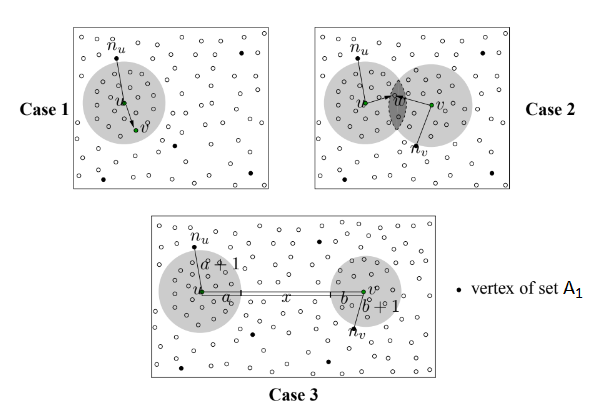
\includegraphics[width=14cm]{images/placeholder_distancequery}
    \centering
    \caption{Placeholder for $\mathbf{dist}(u, v)$}
\end{figure}

\begin{lemma}
    The distance returned by $\mathbf{dist}(u, v)$ is not less than $\delta(u,v)$ and at most $2 * \delta(u,v) + h$.
\end{lemma}
\begin{proof}
    We will go through each of cases
    \begin{enumerate}
        \item \underline{$u \in B_{A_1}(v)$ or $v \in B_{A_1}(u)$:}\newline
            Our structure stores the $B_{A_1}(w)$, $\delta(w, q)$ for $w \in V$, $q \in B_{A_1}(w)$. Exact distance is returned.
            \newpage
        \item \underline{$B_{A_1}(u) \cap B_{A_1}(v) \neq \emptyset$:}\newline
            Since last case did not occur, $u \notin B_{A_1}(v)$ and $v \notin B_{A_1}(u)$ we have $\delta(u,v) \geq \delta(u, A_1)$ and $\delta(u,v) \geq \delta(v, A_1)$.
            Let $w \in B_{A_1}(u) \cap B_{A_1}(v)$, we see that $\delta(u, w) < \delta(u, A_1)$, $\delta(v, w) < \delta(v, A_1)$,
            so $\delta(u, w) + \delta(w, v) < \delta(u, A_1) + \delta(v, A_1) \leq \delta(u,v) + \delta(u,v)$
            $\delta(u, w)$, $\delta(w, v)$ are stored in our structure.
            \newline
            Note that for $u,v,w \in V$ we have
            $$w \in B_{A_1}(u) \cap B_{A_1}(v) \implies u,v \in C_{A_1}(w) \implies \mathcal{O}(u,v)~\text{is defined}$$
            $$\mathcal{O}(u, v) = w \implies u,v \in C_{A_1}(w) \implies w \in B_{A_1}(u) \cap B_{A_1}(v)$$
            so we can retrieve $w \in B_{A_1}(u) \cap B_{A_1}(v)$ from $\mathcal{O}(u,v)$ or tell that $B_{A_1}(u) \cap B_{A_1}(v) = \emptyset$ otherwise.

            For unweighted graphs we can remember exact $\delta(u, v)$ by choosing $w = \mathcal{O}(u,v)$ such that it is on the shortest path from $u$ to $v$.
            Such $w$ exists in unweighted graphs as the shortest path is the one with the least vertices and first $\delta(u, A_1)$ vertices, last $\delta(v, A_1)$ vertices of a path from $u$ to $v$ will be in corresponding balls.
            This also allows us to skip the first case as \newline
            $u \in B_{A_1}(v) \implies v \in B_{A_1}(v)$ for $v \in V$.
        \item \underline{None of the above:}\newline
            Let $x = \delta(B_{A_1}(u), B_{A_1}(v))$, $a = \delta(u, A_1)$, $b = \delta(v, A_1)$.
            Since $B_{A_1}(u) \cap B_{A_1}(v) = \emptyset$ we have $x > 0$.
            Moreover $a + b - h \leq \delta(u,v) < a + b + x$ as any vertices $w \in B_{A_1}(u)$, $q \in B_{A_1}(v)$ realizing
            $\delta(w, q) = x$ are also satisfying $a \leq \delta(u, q)$, $b - h \leq \delta(q, v)$, $\delta(u, w) < a$ and $\delta(v, q) < b$.
            \newline
            Without the loss of generality we assume that $a \leq b$. We then have 
            $$\delta(u, v) ~\leq~ \delta(u, p_{A_1}(v)) + \delta(p_{A_1}(v), v) ~\leq~ 2*\delta(u, p_{A_1}(v)) + \delta(u, v) ~=$$
            $$=~ 2a + \delta(u,v) ~\leq~ (a + b - h) + h + \delta(u,v) ~\leq~ 2*\delta(u, v) + h$$
            $p_{A_1}(v) \in A_1$ so distances from $p_{A_1}(v)$ to all other vertices are stored in our structure.


    \end{enumerate}
\end{proof}

\begin{remark}
    This Oracle is a stretch $2$ Oracle for all cases except for part of case 3.
    For distance estimate $\hat{\delta}(u, v)$, $u,v \in V$ to be more than $2*\delta(u,v)$
    the following must be true: distance is reported at case $3$ and $\delta(u, v) < 2*\delta(u, p_{A_1}(u))$ as our error is at most $2*\delta(u, p_{A_1}(u))$, so
    both of the below must be true:\newline
    $\delta(p_{A_1}(u), v) < 3*\delta(u, p_{A_1}(u))$ and $\delta(p_{A_1}(v), u) < 3*\delta(v, p_{A_1}(v))$
    \newline
    Those conditions could be easily verified during Oracle query.
\end{remark}

We can make even stronger argument, the Oracle is not a stretch $2$ only if the balls of the queried vertices have no common vertex, but they are connected by a single edge.
This however can not be verified by this Oracle.


\section{Improved Sampling Algorithm}

\noindent\fbox{
    \begin{minipage}{\textwidth -14.1pt}
    algorithm $\mathbf{sample}(X, p)$

    $R \leftarrow \emptyset ; X' \leftarrow X$

    while $X' \neq \emptyset$

    ~~~~Let $S$ be an uniform sample from $X'$ of size $\ceil[\big]{p * |X|}$ or $X'$ if $\ceil[\big]{p * |X|} > |X'|$

    ~~~~$R \leftarrow R \cup S$

    ~~~~For every $v \in X'$

    ~~~~~~~~calculate $C_R(v) \cap X$

    ~~~~$X' \leftarrow \{v \in X ~|~ |C_R(v) \cap X| > 4/p \}$

    return $R$

    \end{minipage}
}

\begin{remark} \label{clusterSize}
The algorithm $\mathbf{sample}(X, p)$ ensures that all $C_R(v)$ clusters have at most $4/p$ vertices, so all $C_{A_1}(v)$ clusters have at most $4/p$ vertices.
This ensures that $\mathcal{O}$ have at most $16n/p^2$ defined values.
\end{remark}

\begin{lemma} \label{algSampleLogSteps}
    In each step of sample $\mathbf{sample}(X, p)$, the $|X'|$ is at least halved with probability at least $1/2$.
\end{lemma}

\begin{proof}
    Let $X_i$ be the set $X'$ at the beginning of $i$-th step. Note that $X_i \supseteq X_{i+1}$ as $R$ never shrinks so clusters $C_R$ never grow larger.
    If $|X_i| < \ceil[\big]{p * |X|}$ then $|X_{i+1}| = 0$ and lemma holds.
    In other case after the set $R$ is augmented by sample $S$ ($R \supseteq S$) we note that
    

    $$\sum_{v \in X_i} |C_R(v) \cap X| = \sum_{v \in X} |B_R(v) \cap X_i| \leq \sum_{v \in X} |B_S(v) \cap X_i| $$
    by Lemma \ref{ballSize}
    $$\mathbf{E}[\sum_{v \in X} |B_S(v) \cap X_i|] < |X| * (p * |X|/|X_i|)^{-1} = |X_i|/p$$

    By Markov inequality with probability $1/2$ we have $\sum_{v \in X_i} |C_R(v) \cap X| < 2|X_i|/p$,
    and since in that case 
    $$|X_{i+1}| * 4/p \leq \sum_{v \in X_i} |C_R(v) \cap X| < 2|X_i|/p$$
    so $2 * |X_{i+1}| < |X_i|$ with probability at least $1/2$.

\end{proof}

So the expected number of steps is at most $2$ log $n$

By combining above Lemma with Lemma \ref{ballSize} we can prove the following Lemma

\begin{lemma} \label{sampleAlg}
    Given an undirected \underline{weighted} graph with non-negative weights, a set $X$, $X \subseteq V$ and number $0 < p < 1$, we can compute a sample set
    $R$ of expected size $O(p*|X|$~log~$|X|)$ such that for every $v \in V$ $C_R(v) \cap X$ is of size at most $4/p$ and expected size of $B_R(v) \cap X$ is less than $1/p$.
\end{lemma}


\section{Efficient Ball and Cluster Computation}

\begin{lemma} \label{ballClusterComputation}
    Given an undirected \underline{weighted} graph with non-negative weights, number $0 < p < 1$ and set $A_1$ generated by algorithm $\mathbf{sample}(V, p)$,
    we can calculate $B_{A_1}(v)$, $C_{A_1}(v)$ and $\delta(v,u)$ for every $v \in V$, $u \in B_{A_1}(v)$ in $O(m/p + n/p $ log $n )$ time.
\end{lemma}

\begin{proof}
    We start by calculating the $\delta(v, A_1)$ for every $v \in V$. We can do this by adding to the graph a source vertex $s$ and connecting it to every $u \in A_1$ by edge of weight $0$, and then
    running the Dijkstra algorithm from there. It is not hard to see that this will calculate $\delta(v, A_1)$ for every $v \in V$ in $O(m + n $ log $n)$ time.
    
    Now for every $v \in V$ we know the $\delta(v, A_1)$, so
    we can run modified Dijkstra algorithm to calculate $B_{A_1}(v)$ and $\delta(v, u)$ for $u \in B_{A_1}(v)$.
    We modify Dijkstra algorithm to ignore edges that lead to too far away vertices $-$ vertices $u \in V$ such that $\delta(v,u) \geq \delta(v, A_1)$.
    Such modified Dijkstra will work in $O(\xi(B_{A_1}(v)) + |B_{A_1}(v)| $ log $|B_{A_1}(v)|)$ time, where $\xi(X)$, $X \subseteq V$
    is the number of edges incident to vertices of $X$.
    
    \begin{remark} \label{ballClusterEquivalence}
    Note that when $B_{A_1}(v)$ is calculated for every $v \in V$, we can easily calculate $C_{A_1}(v)$ as $u \in B_{A_1}(v) \iff v \in C_{A_1}(u)$, $u \in V$.
    This will not change the time complexity as $\sum_{v \in V}|B_{A_1}(v)| = \sum_{v \in V}|C_{A_1}(v)|$
    \end{remark}

    The Mikkel Thorup claims that his algorithm can be modified in a similar way (at least for calculating clusters) \cite{a0OraclesBasic},
    achieving working time of $O(\xi(B_{A_1}(v)) + |B_{A_1}(v)|) = O(\xi(B_{A_1}(v)))$.

    Lets calculate an upper bound on $\sum_{v \in V} \xi(B_{A_1}(v))$:

    $$\sum_{v \in V} \xi(B_{A_1}(v)) = \sum_{v \in V} \sum_{u \in B_{A_1}(v)} \xi(u) =$$
    $$= \sum_{u \in V} \sum_{v \in C_{A_1}(u)} \xi(u) =$$
    $$= \sum_{u \in V} |C_{A_1}(u)|\xi(u) \leq \sum_{u \in V} 4\xi(u)/p \leq 8m/p $$ 

    So the total working time of the above is 
    \newline
    $O(m + n $ log $ n + 8m/p + \sum_{v \in V}|B_{A_1}(v)| $ log $|B_{A_1}(v)|) =$
    \newline
    $=O(m/p + n/p $ log $n) $

\end{proof}

The above weighted graphs Ball and Cluster computation requires the clusters to be bounded by their size, without it the bound on computation time will increase.

\begin{remark} \label{ballClustersForUniformSample}
    If $A_1$ would be a set containing uniform sample from $V$ of size $\ceil[\big]{p * |V|}$ instead, then the expected size of $\sum_{v \in V} \xi(B_{A_1}(v))$ would be bounded by Lemma \ref{ballSize} and since $B_X(v) \leq B_Y(v)$ for $X \subseteq Y \subseteq V$, $v \in V$
    $$\sum_{u \in V} |C_{A_1}(u)|\xi(u) \leq \sum_{u \in V} |C_{A_1}(u)| * n = n * \sum_{u \in V} |C_{A_1}(u)| = n * \sum_{v \in V} |B_{A_1}(v)| \leq n^2/p$$
    Which changes the computation time from deterministic $O(m/p + n/p $ log $n) $ to expected $O(n^2/p)$.
\end{remark}

For undirected graphs however, computation is much simpler and will work for
$\mathbf{sample}(V, p)$

\begin{figure}[h]
    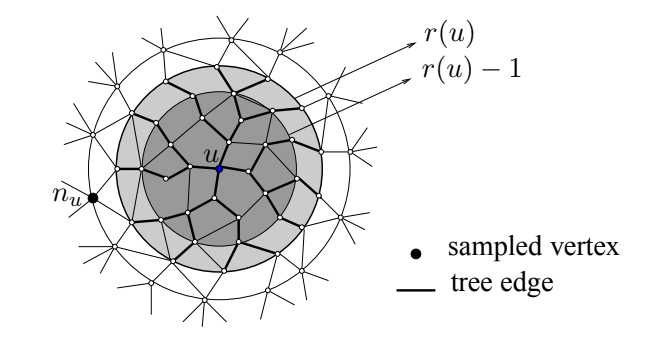
\includegraphics[width=10cm]{images/placeholder_unweightedball}
    \centering
    \caption{Placeholder for unweighted ball computation}
\end{figure}

\begin{lemma} \label{ballClusterUnweighted}
    Given an undirected \underline{unweighted} graph with no multiple edges, number $0 < p < 1$ and
    uniform sample $S$ from $V$ of size $\ceil[\big]{p * |V|}$
    we can calculate $B_{S}(v)$ and $C_{S}(v)$ for every $v \in V$ in $O(m + n/p^2)$ expected time.
\end{lemma}

\begin{proof}
    First we compute $\delta(v, S)$ for every $v \in V$. This can be done in $O(m)$ time by a single BFS traversal.
    We do that by adding a source vertex $s$ that is connected to every $u \in S$ and starting BFS in that vertex.
    Indeed, if $\delta(v, S) = x$ then $\delta(v, u) = x - 1$ for some $u \in S$ and $\delta(v, w) \geq x - 1$ for every $w \in S$, so
    $\delta(v, s) = \delta(v, S) + 1$

    Now for every $v \in V$ we compute ball $B_{S}(v)$ using BFS, we immediately halt the edge processing when we reach a vertex $u \in V$ such that $\delta(v,S) - 1 \leq \delta(v, u)$.
    That way we are guaranteed to visit every $w \in V$ such that $\delta(v, w) \leq \delta(v, S) - 1$, but
    we will not process any edges from vertices $q \in V$ such that $\delta(v, q) \geq \delta(v, S) - 1$ (Unless the edge was processed by a vertex visited earlier).

    Lets count the expected number of edges processed. Let $u \in V$ be any vertex and
    $v_1, v_2, \ldots, v_n \in V$ be vertices of $V$ arranged in BFS non-decreasing order of distance from $u$.
    Each edge will be processed at most twice, from both (or one) of vertices it is connecting. We will count only the first time $-$ when the edge is connecting to the vertex that was not visited (or when edge is a loop).
    The BFS can process the edges of $v_i$ when both of the below conditions are satisfied (required, but not sufficient):
    \begin{enumerate}
        \item $\psi_1^i$: There is no vertex in the set $\{v_j |0 < j < i\}$ which is selected in the sample $S$.
        \item $\psi_2^i$: There is no vertex in the set $\{v_j |i \leq j \leq n\}$ that is in $S$ and there is edge between it and $v_i$.
    \end{enumerate} 
    The chance for the $\psi_1^i$ is no more than $(1-p)^{i-1}$ as the chance for $v_j \in S$ is $\ceil[\big]{p * |V|}/|V| \geq p$.
    
    If $\psi_1^i$ is true then chance for $\psi_2^i$ is no more than
    \newline
    $(1 - $Pr$[v_j \in S $ for $i < j \leq n ~|~ \psi_1^i])^{\xi'(v_i)}$, where $\xi'(v_i)$ is number of edges connecting $v_i$ with any $v_j$ where $i \leq j \leq n$.
    \newline
    Pr$[v_j \in S $ for $i < j \leq n ~|~ \psi_1^i] > p$ as $\psi_1^i$ for $i < j \leq n$ increase the chance for $v_j \in S$ that was originally $\ceil[\big]{p * |V|}/|V| \geq p$.
    That gives Pr$[\psi_2^i ~|~ \psi_1^i] \leq (1-p)^{\xi'(v_i)}$
    \newline
    Now lets look at the expected number of edges processed at least once $-$ it is no more than
    $$\sum_{i=1}^{n} \text{Pr}[\psi_1^i] * \text{Pr}[\psi_2^i ~|~ \psi_1^i] * \xi'(v_i) \leq \sum_{i=1}^{n} ((1-p)^{i-1} (1-p)^{\xi'(v_i)}\xi'(v_i)) \leq$$
    $$\leq \sum_{i=1}^{n} ((1-p)^{i-1} \sum_{j=1}^{\xi'(v_i)}(1-p)^{j-1}) \leq 
    \sum_{i=1}^{n} ((1-p)^{i-1} * 1/p) \leq 1/p * \sum_{i=1}^{n} ((1-p)^{i-1}) \leq 1/p^2$$

\end{proof}


\section{Preprocessing Memory and Time}

We first compute the $\mathbf{sample}(V, p)$ which consists of while loop with expected $2$ log $n$ iterations,
in each one we compute uniform sample $S$ in time $O(n)$, and then $B_R(v)$, $C_R(v)$ for $v \in V$, where $R$ contains uniform sample from $V$ of size $\ceil[\big]{p * |V|}$.
This can be done by Lemma \ref{ballClusterComputation} and by Observation \ref{ballClustersForUniformSample} for weighted graphs or by Lemma \ref{ballClusterUnweighted} for unweighted graphs.
We can compute the $B_R(v)$ in $O(m + n^2/p)$ expected time for weighted graphs or $O(m + n/p^2)$ expected time for unweighted graphs.
The calculation of clusters and their sizes can be done by Observation \ref{ballClusterEquivalence} without affecting the complexity.
The total expected time is $O(m $ log $ n + n^2/p $ log $ n)$ for weighted graphs or $O(m $ log $ n + n/p^2 $ log $ n)$ for unweighted graphs.
The balls and clusters have expected size of $O(1/p)$ so they will not take more than $O(n/p $ log $ n)$ expected auxiliary memory.

We can compute $\delta(u,v)$, $p_{A_1}(v)$ for every $u \in A_1$, $v \in V$ by running Dijkstra algorithm for each of the $u \in A_1$.
However will take $O(|A_1| *(m + n$ log $ n))$ time.
We can do this faster, in $O(m|A_1|) = O(mnp$ log$ n)$, by using efficient Thorup algorithm for undirected graphs with floating point edge weights \cite{uberDijkstraInt}\cite{uberDijkstraFloat}.
For unweighted graphs a simple BFS will be enough.
Finding $p_{A_1}(v)$ can be done afterwards by checking every distance calculated.
The expected auxiliary memory is $O(n|A_1|) = O(n^2p$ log$ n)$.

Next we will compute balls and clusters using Lemma \ref{ballClusterComputation} in $O(m/p + n/p $ log $ n)$ expected time and $O(n/p)$ deterministic auxiliary memory.

And at the end we will compute $\mathcal{O}$ in $O(n/p^2)$ memory as cluster size is bounded by $4/p$ (Observation \ref{clusterSize}).
The time could be either expected $O(n/p^2)$ or deterministic $O(n/p^2 $ log $ n)$ depending on hash table construction method used.

This will total to $O(m $ log $ n + n^2/p $ log $ n + mnp$ log $ n + m/p + n/p $ log $ n + n/p^2) = O(n^2/p $ log $ n + mnp$ log $ n + n/p^2)$ expected time for weighted graphs
or $O(n/p^2 $ log $n + mnp $ log $n)$ expected time for unweighted graphs.

The expected auxiliary memory is $O(n/p $ log $ n + n^2p$ log$ n + n/p + n/p^2) = O(n^2p$ log$ n + n/p^2)$.

For $p = n^{-1/3}$ and $m \geq n$ the expected auxiliary memory is the lowest $-$ $O(n^{5/3} $ log $ n)$.
The expected time is then $O(n^{7/3} $ log $ n + mn^{2/3}$ log $ n)$ for weighted graphs and
$O(mn^{2/3}$ log $ n)$ for unweighted graphs. For $m = O(n^2)$ the expected time is $O(n^{8/3} $ log $n)$ in both cases.

By Markov inequality we can get deterministic auxiliary memory $O(n^{5/3} $ log $ n)$ in expected constant number of $\mathbf{prepro}(G)$ executions.

\begin{remark}
As Oracle uses only data structures that were generated during preprocessing the auxiliary preprocessing memory is an upper bound on the oracle memory.
\end{remark}






\chapter{Removing the Log Factors} \label{21TheoreticalComparison}

\section{Oracle by Mihai Patrascu and Liam Roditty} \label{21OraclePatRod}

We present the slightly modified $(2,1)-approximate$ distance oracle of Mihai Patrascu and Liam Roditty \cite{21OracleLessMemory}

\noindent\fbox{
    \begin{minipage}{\textwidth -14.1pt}
    algorithm $\mathbf{preproPatRod}(G)$

    let $R$ be an uniform sample from $V$ of size $\ceil[\big]{n^{-1/3} * n}$ 
    
    let $S$ be an uniform sample from $V$ of size $\ceil[\big]{n^{-2/3} * n}$

    let $A_1 \leftarrow R \cup \bigcup_{u \in S} B_R(u)$

    for every $u \in A_1$

    ~~~~for every $v \in V$
    
    ~~~~~~~~calculate $\delta(u,v)$

    for every $v \in V$

    ~~~~calculate $p_{A_1}(v)$, $B_{A_1}(v)$ and $C_{A_1}(v)$

    ~~~~for every $u \in B_{A_1}(v)$

    ~~~~~~~~calculate $\delta(v,u)$

    ~~~~for every pair $ (u,w) \in C_{A_1}(v) \times C_{A_1}(v)$

    ~~~~~~~~$\mathcal{O}(u,w) \leftarrow v$

    \end{minipage}
}

The only difference between this Oracle and Oracle from chapter \ref{21DistanceOracle} is that this oracle
constructs $A_1$ by adding $B_R(u)$, $u \in S$ to the set $R$, instead of adding \~log $n$ sets of size $R$ to the set $R$, which reduces the memory complexity by log $n$.
Here we get a weaker bound on $C_{A_1}(v)$, $v \in V$, which fortunately is claimed to not increase preprocessing time for sparse graphs too much \cite{21OracleSpannerNoPenaltyNoLog}.

\begin{lemma} \label{patRodBallIntersections}
    There is at most $O(n^{5/3})$ expected pairs of vertices $(u, v) \in V \times V$
    such that $B_{A_1}(u) \cap B_{A_1}(v) \neq \emptyset$,
    if $A_1$ was constructed by $\mathbf{preproPatRod}(G)$.
\end{lemma}

\begin{proof}
    We will proof the Lemma by showing that for $u \in V$ expected number of balls intersecting with $B_{A_1}(u)$ is less than $n^{2/3}$.

    The program generates first the sample $R$.
    Let $u_1, u_2, \ldots, u_n$ be the elements of $V$ arranged in any non-decreasing order of distance from $u$.

    Now let $w_1, w_2, \ldots, w_n$ be the elements of $V$ arranged in any order such that if $i \leq j$ then 
    for every $l$ such that $w_j \in C_R(u_l)$ there is such $k$ that $w_i \in C_R(u_k)$ we have $k \leq l$.
    In other words we order the vertices by the first cluster (the one with the smallest $i$) $C_R(u_i)$, $i \in \{1, \ldots, n\}$ that it belongs to.

    Now the program generates the sample $S$. What is the expected size of the set $L = \{w_1, w_2, \ldots, w_l\}$ such that $L \cap S = \emptyset$ and $L$ is largest possible?

    $$\mathbf{E}[|L|] = \sum_{i=1}^{n} \text{Pr}[w_i \in L] =\sum_{i=1}^{n} \text{Pr}[\{w_1, w_2, \ldots, w_i\} \cap S = \emptyset] \leq $$
    $$\leq \sum_{i=1}^{n} \sum_{j=1}^{i} Pr[w_j \notin S] \leq \sum_{i=1}^{n} (1 - n^{-2/3})^i < n^{2/3}$$

    For $v \in V$ we claim that $B_{A_1}(u) \cap B_{A_1}(v) \neq \emptyset \implies v \in L$.

    We prove the claim by contradiction: Suppose that $B_{A_1}(u) \cap B_{A_1}(v) \neq \emptyset$ and $v \notin L$

    We have $v$ = $w_k$ for some $l + 1 \leq k \leq n$. 
    Note that $w_{l+1}$ exists as otherwise $L = V$, $v \in L$ and $w_{l+1} \in S$, as $L$ is largest possible 
    
    Let $u_i$ $1 \leq i \leq n$ be such vertex, that $v \in C_R(u_i)$ and $i$ is smallest possible.
    If no such $u_i$ exists then $\delta(v, R) = 0$ as otherwise $v \in C_R(v)$, however $\delta(v, R) = 0 \implies B_R(v) = B_{A_1}(v) = \emptyset$, contradiction.

    Now let $u_j$ $1 \leq j \leq n$ be such vertex, that $w_{l+1} \in C_R(u_j)$ and $j$ is smallest possible. 
    If no such $u_j$ exists then since $u_i$ exists we have $k < l + 1$, so $v = w_k \in L$.

    Since $k \geq l + 1$ we have $i \geq j$, so $\delta(u, u_i) \geq \delta(u, u_j)$, but $w_{l+1} \in C_R(u_j)$, so $u_j \in B_R(w_{l+1})$ and $w_{l+1} \in S$
    which means that $u_j \in A_1$, so $u_j \notin B_{A_1}(u)$ and $u_i \notin B_{A_1}(u)$.
    However $u_i$ is the closest vertex to $u$ such that $u_i \in B_R(v)$ and since $B_R(v) \supseteq B_{A_1}(v)$, 
    we get a contradiction $B_{A_1}(u) \cap B_{A_1}(v) = \emptyset$.
\end{proof}

\begin{remark}
    The above proof also gives an estimation on expected value of $\sum_{v \in V}|C_{A_1}(v)|^2$.
    Indeed when we look at set $L_u$ ($L$ generated for a given $u$) we see that it contains all elements from clusters $C_R(v)$, where $v \in B_{A_1}(u)$.
    This points to:

    $$\sum_{v \in V}|C_{A_1}(v)|^2 = \sum_{v \in V}\sum_{u \in C_{A_1}(v)}|C_{A_1}(v)| = \sum_{u \in V}\sum_{v \in B_{A_1}(u)} |C_{A_1}(v)| \leq$$
    $$\leq \sum_{u \in V}\sum_{v \in B_{A_1}(u)} L_u = \sum_{u \in V} |B_{A_1}(u)| * L_u \leq \sum_{u \in V} |B_R(u)| * L_u$$
    $$\mathbf{E}[\sum_{v \in V}|C_{A_1}(v)|^2] \leq \mathbf{E}[\sum_{u \in V} |B_R(u)| * L_u] = \sum_{u \in V} \mathbf{E}[|B_R(u)| * L_u] \leq n * n^{1/3} * n^{2/3} = n^2$$
    as our upper bounds on $\mathbf{E}[|B_R(u)|]$ and $\mathbf{E}[L_u]$ are independent $-$ we generate the $B_R(u)$ and $w_1, w_2, \ldots, w_n$ (for a given $u$) based on sample $R$ and graph $G$
    and then we generate random sample $S$ that gives us $L_u$ together with its upper bound, while $B_R(u)$ remains unaffected
\end{remark}

It is claimed that the calculation of the hash table $\mathcal{O}$ is possible in $O(mn^{2/3})$ \cite{21OracleSpannerNoPenaltyNoLog}

The generation of $R$ and $S$ takes $O(n)$,
the computation $B_R(u), u \in S$ takes $O(m + |S|/p^2) = O(m + n)$ expected time as stated by Lemma \ref{ballClusterUnweighted}.
The computation of $A_1$ then happens in $O(n)$ time. The expected auxiliary memory is $O(n)$.
We see that the generation $A_1$ is very fast and the expected size of $A_1$ is $O(n^{2/3})$
as $|R| = \ceil[\big]{n^{2/3}}$, $|S| = \ceil[\big]{n^{1/3}}$ and expected size of $B_R(u), u \in S$ is less than $n^{1/3}$ by Lemma \ref{ballSize}.

The calculation of $\delta(u,v)$, $p_{A_1}(v)$ for every $u \in A_1$, $v \in V$ takes only expected $O(mn^{2/3})$ time and $O(n^{5/3})$ expected auxiliary memory.
This is an improvement by the factor of log $n$.

The expected value of $\sum_{v \in V}|C_{A_1}(v)|^2$ is $n^2$, so the computation of $\mathcal{O}$ takes $O(n^2)$ expected time.
The expected auxiliary memory remains at $O(n^{5/3})$ thanks to Lemma \ref{patRodBallIntersections}.

The total expected time is $O(n^{2} + mn^{2/3})$ (or $O(mn^{2/3})$ by claim from \cite{21OracleSpannerNoPenaltyNoLog}), expected auxiliary memory $O(n^{5/3})$.

\section{Further Improvements}

The Oracle preprocessing time could be further improved to $O(n^2)$ by applying spanners $-$ subgraphs of a graph that have less edges than original
but the distances between nodes are preserved up to some error (usually additive or multiplicative).
This however comes with the drawbacks as either the distance approximation is worse $-$ stretch $(2,3)$ \cite{21OracleBasic} or the oracle becomes more complicated \cite{21OracleSpannerNoPenalty} \cite{21OracleSpannerNoPenaltyNoLog}
However using spanners will only improve the preprocessing time for graphs with $\omega(n^{4/3})$ edges, as currently known construction of good enough spanner takes $\Theta(n^2)$ time.

The Oracle can be generalized similar to Oracle from Chapter \ref{30DistanceOracle} to produce $(2k - 2, 1)-approximate$ distance oracle of size $O(n^{1 + 2/(2k-1)})$ \cite{a1Oracle}

The are also more efficient algorithms for the special classes of graphs $-$ sparse graphs, planar graphs.


\chapter{Results} \label{21PracticalComparison}

\section{Perfect Hashing Functions Generation}

\begin{definition}
    A minimal perfect hash function is a function that given a set of keys $S$ maps them bijectively to into the set $\{1,2,\ldots,|S|\}$.
\end{definition}

In the following we will call minimal perfect hash functions simply a perfect hash functions.

The hash table used in the programs is PTHash \cite{hashTablePractical}, minimal perfect hash algorithm
The implementation of PTHash is written in C++ and available at
\newline 
\url{https://github.com/jermp/pthash}

The construction time of PTHash is superlinear, fortunately this will not affect the time complexity as all algorithm use $\Omega(n^2)$ preprocessing time,
but only $O(n^{5/3})$ write operations. However, the practical construction time should improve as PTHash is very efficient.

\section{Programs Compared}

The first program marked as $\mathbf{BFS}$ compared is an Oracle with $A_1 = V$, 
every exact distance is calculated by $BFS$ algorithm and stored in memory.
This is our control sample.

The second program $\mathbf{Basic}$ is an Oracle with $A_1$ being an uniform sample from $V$ of size $\ceil[\big](p*|V|) = \ceil[\big](n^{2/3})$.
Its the most basic $(2,1)$ Distance Oracle without any expansion of the $A_1$ that would ensure small number of ball intersections.
This Oracle have expected memory of $\Omega(n^{7/3})$ for some graphs.

The third program $\mathbf{BasGoySen}$ is Chapter \ref{21DistanceOracle}. Sample $A_1$ is expanded by vertices with big clusters until none remains.

The fourth and the last program $\mathbf{PatRod}$ is Chapter \ref{21TheoreticalComparison} section \ref{21OraclePatRod} Oracle. Sample $A_1$ is expanded by random balls.

As the programs are very similar, we run the same tests with the same seed for all random sampling (different tests have different seeds).
This ensures that the first sample will be the same for all programs, removing some noise from our comparison.
However we have made no attempt to modify the PTHash code, so the perfect hash functions generated are different with each run.



\section{Random Graphs Comparison}

The Oracles were tested on random graphs with $n = 2000 \pm 100$ in order to avoid any distortions from dense graphs with particular number of vertices, such as program behaving differently on semi-clique graphs with even or odd number of vertices.
The number of edges was randomly chosen from $n^a(n - 1)/10$ to $n^a(n-1)/2$ for a parameter $0 \leq a \leq 1$.
Edges themselves were an uniform sample from all possible edges (no loops and multiple edges).

The following quantities were measured:
\begin{itemize}
    \item Preprocessing Time $-$ Time taken (in seconds) from the moment after input was loaded into memory to the moment oracle is ready to answer queries.
    \item Average Query Time $-$ Time taken (in seconds) to report $\hat{\delta}(u, v)$, for every $u, v \in V$ divided by $|V|^2$.
    \item Size of the Set $A_1$ $-$ self explanatory.
    \item $n*|A_1|$ $-$ Memory needed (in machine words) to store $\delta(u, v)$, for every $u \in A_1$, $v \in V$.
    \item Sum of Ball sizes $-$ $\sum_{v \in V} |B_{A_1}(v)| = \sum_{v \in V} |C_{A_1}(v)|$ $-$ Memory needed (in machine words) to store $\delta(v, u)$, for every $v \in V$, $u \in B_{A_1}(v)$.
    \item Space PHFs $B_{A_1}$ $-$ Memory needed (in bits) to store the perfect hash function for every $B_{A_1}(v)$, $v \in V$ that allows to access any ball element in constant time, while not using additional memory. 
            The hash function generator seems to struggle with low key numbers, hence large number of bits for empty balls. This could be fixed by combining all functions into one, if needed.
    \item Space PHFs $\mathcal{O}$  $-$ Memory needed (in bits) to store the perfect hash function for table $\mathcal{O}$.
    \item Average Relative Error $-$ Arithmetic average of errors calculated\newline 
            as $(\hat{\delta(u,v)} - \delta(u,v)) / \delta(u,v)$.
            If $\delta(u,v) = 0$ or there is no path between $u$ and $v$, all oracles recognize it flawlessly and hence the error is $0$.
    \item Worst Error percentage $-$ The number of times the reported distance was $2*\delta(u, v) + 1$ divided by number of all distances reported.
\end{itemize}

\begin{table}[H] \label{test:random.a10}
    \centering
    \begin{tabular}{ |p{3cm}||p{2cm}|p{2cm}|p{2cm}|p{2cm}|  } 
        \hline
        & $\mathbf{BFS}$ & $\mathbf{Basic}$ & $\mathbf{BaGoSe}$ & $\mathbf{PatRod}$ \\
        \hline
        \hline
        Preprocess Time                 & 42.2736    & 3.4243     & 3.4170      & 3.6729     \\
        \hline
        Avg. Query Time                 & 1.3815e-07 & 1.4916e-07 & 1.5012e-07  & 1.5001e-07 \\
        \hline
        $|A_1|$                         & 1993.3     & 158.9      & 158.9       & 171.1      \\
        \hline
        $n * |A_1|$                     & 3.9756e+06 & 316860     & 316860      & 341175     \\
        \hline
        $\sum_{v \in V} |B_{A_1}(v)| $  & 0          & 1834.4     & 1834.4      & 1822.2     \\
        \hline
        $|\mathcal{O}|$                 & 0          & 1834.4     & 1834.4      & 1822.2     \\
        \hline
        Space PHFs $B_{A_1}$            & 6.4035e+06 & 6.4041e+06 & 6.4043e+06  & 6.4041e+06 \\
        \hline
        Space PHFs $\mathcal{O}$        & 3216       & 13638.4    & 13644.8     & 13558.4    \\
        \hline
        Average Error                   & 0          & 0.6674     & 0.6674      & 0.6584     \\
        \hline
        Worst Error (\%)                & 0          & 10.4053    & 10.4053     & 10.2423    \\
        \hline
        Total Space                     &            &            &             &            \\
        \hline

    \end{tabular}
    \caption{$n = 2000 \pm 100$, $a = 1.0$, Random Graph, arithmetic average of $10$ tests}
\end{table}

The very dense random graphs $-$ $a=1.0$ with at least $1/5$ of all possible edges have all or almost all balls and clusters of size $\leq 1$.
The preprocessing time is the largest here especially for the naive $\mathbf{BFS}$ approach.
The oracle reports the approximate with over $10\%$ of answers being reported with bigger stretch than $2$. The average reported distance is $\sim 66 \%$ greater than real distance.
The errors are surprisingly large considering that most if not all distances are not larger than $2$.

\begin{table}[H] \label{test:random.a0.75}
    \centering
    \begin{tabular}{ |p{3cm}||p{2cm}|p{2cm}|p{2cm}|p{2cm}|  } 
        \hline
        & $\mathbf{BFS}$ & $\mathbf{Basic}$ & $\mathbf{BaGoSe}$ & $\mathbf{PatRod}$ \\
        \hline
        \hline
        Preprocess Time                 & 6.2580     & 0.5368     & 0.5411      & 0.5764     \\
        \hline
        Avg. Query Time                 & 1.3829e-07 & 1.5242e-07 & 1.5335e-07  & 1.5128e-07 \\
        \hline
        $|A_1|$                         & 1998.3     & 159.2      &  159.2      & 171.1      \\
        \hline
        $n * |A_1|$                     & 3.9954e+06 & 318240     &  318240     & 342014     \\
        \hline
        $\sum_{v \in V} |B_{A_1}(v)| $  & 0          & 1892.2     & 1892.2      & 1857.9     \\
        \hline
        $|\mathcal{O}|$                 & 0          & 2010.2     & 2010.2      & 1921.9     \\
        \hline
        Space PHFs $B_{A_1}$            & 6.4194e+06 & 6.4206e+06 & 6.4207e+06  & 6.4208e+06 \\
        \hline
        Space PHFs $\mathcal{O}$        & 3216       & 13188.8    & 14188.8     & 13902.4    \\
        \hline
        Average Error                   & 0          & 0.4681     & 0.4629      & 0.4629     \\
        \hline
        Worst Error (\%)                & 0          & 6.1077     & 6.0448      & 6.0448     \\
        \hline
        Total Space                     &            &            &             &            \\
        \hline

    \end{tabular}
    \caption{$n = 2000 \pm 100$, $a = 0.75$, Random Graph, arithmetic average of $10$ tests}
\end{table}

The slightly less dense random graphs $-$ $a=0.75$ have some of the balls intersecting, much better preprocessing time by about the same factor $6.7$ for all programs.
And smaller errors both average and percent of worst case by about factor of $2/3$.


\begin{table}[H] \label{test:random.a0.5}
    \centering
    \begin{tabular}{ |p{3cm}||p{2cm}|p{2cm}|p{2cm}|p{2cm}|  } 
        \hline
        & $\mathbf{BFS}$ & $\mathbf{Basic}$ & $\mathbf{BaGoSe}$ & $\mathbf{PatRod}$ \\
        \hline
        \hline
        Preprocess Time                 & 0.9339     & 0.1373     & 0.1399      & 0.1399     \\
        \hline
        Avg. Query Time                 & 1.3671e-07 & 1.9346e-07 & 1.9343e-07  & 1.7201e-07 \\
        \hline
        $|A_1|$                         & 1995.9     & 159        & 159         & 205.1      \\
        \hline
        $n * |A_1|$                     & 3.9849e+06 & 317416     & 317416      & 409890     \\
        \hline
        $\sum_{v \in V} |B_{A_1}(v)| $  & 0          & 6785.7     & 6785.7      & 4650.3     \\
        \hline
        $|\mathcal{O}|$                 & 0          & 32557.1    & 32557.1     & 16005.1    \\
        \hline
        Space PHFs $B_{A_1}$            & 6.4119e+06 & 6.4399e+06 & 6.4396e+06  & 6.4208e+06 \\
        \hline
        Space PHFs $\mathcal{O}$        & 3196.8     & 131400     & 130677      & 13902.4    \\
        \hline
        Average Error                   & 0          & 0.3012     & 0.3012      & 0.2796     \\
        \hline
        Worst Error (\%)                & 0          & 0.9458     & 0.9458      & 0.9842     \\
        \hline
        Total Space                     &            &            &             &            \\
        \hline

    \end{tabular}
    \caption{$n = 2000 \pm 100$, $a = 0.5$, Random Graph, arithmetic average of $10$ tests}
\end{table}

For random graphs with about $n^{3/2}$ edges $-$ $a = 0.5$ the $\mathbf{BFS}$ speeds up again by a factor $\sim 6.7$, however other programs
speed up about $4$ times as the balls here starts to intersect in bigger numbers.
As balls grow in size the Worst Error Percentage drops rapidly, while the average error drops again by factor $\sim 2/3$

\begin{table}[H] \label{test:random.a0.25}
    \centering
    \begin{tabular}{ |p{3cm}||p{2cm}|p{2cm}|p{2cm}|p{2cm}|  } 
        \hline
        & $\mathbf{BFS}$ & $\mathbf{Basic}$ & $\mathbf{BaGoSe}$ & $\mathbf{PatRod}$ \\
        \hline
        \hline
        Preprocess Time                 & 0.2460     & 0.1500     & 0.1554      & 0.1082     \\
        \hline
        Avg. Query Time                 & 1.4172e-07 & 2.6281e-07 & 2.6099e-07  & 1.9993e-07 \\
        \hline
        $|A_1|$                         & 1972.2     & 157.8      & 157.8       & 234.7      \\
        \hline
        $n * |A_1|$                     & 3.8929e+06 & 311392     & 311392      & 464122     \\
        \hline
        $\sum_{v \in V} |B_{A_1}(v)| $  & 0          & 12177.8    & 12177.8     & 8636.1     \\
        \hline
        $|\mathcal{O}|$                 & 0          & 122816     & 122816      & 63118.9    \\
        \hline
        Space PHFs $B_{A_1}$            & 6.3360e+06 & 6.3941e+06 & 6.3942e+06  & 6.3736e+06 \\
        \hline
        Space PHFs $\mathcal{O}$        & 3216       & 301478     & 299878      & 167926     \\
        \hline
        Average Error                   & 0          & 0.1751     & 0.1751      & 0.1393     \\
        \hline
        Worst Error (\%)                & 0          & 0.2024     & 0.2024      & 0.1562     \\
        \hline
        Total Space                     &            &            &             &            \\
        \hline

    \end{tabular}
    \caption{$n = 2000 \pm 100$, $a = 0.25$, Random Graph, arithmetic average of $10$ tests}
\end{table}

For $a = 0.25$ the random graphs have a lot of balls intersecting, which causes the $\mathbf{Basic}$ and $\mathbf{BaGoSe}$
to work slower despite the better theoretical complexity for $\mathbf{BaGoSe}$.
Here the $\mathbf{PatRod}$ is faster then the rest of algorithms, despite being similar on other tests.
The Average Error drops as usual.

\begin{table}[H] \label{test:random.a0}
    \centering
    \begin{tabular}{ |p{3cm}||p{2cm}|p{2cm}|p{2cm}|p{2cm}|  } 
        \hline
        & $\mathbf{BFS}$ & $\mathbf{Basic}$ & $\mathbf{BaGoSe}$ & $\mathbf{PatRod}$ \\
        \hline
        \hline
        Preprocess Time                 & 0.0428     & 0.0464     & 0.0484      & 0.0471     \\
        \hline
        Avg. Query Time                 & 1.1239e-07 & 1.2350e-07 & 1.2445e-07  & 1.2298e-07 \\
        \hline
        $|A_1|$                         & 2008.9     & 159.7      & 159.7       & 181.5      \\
        \hline
        $n * |A_1|$                     & 4.0401e+06 & 321056     & 321056      & 364936     \\
        \hline
        $\sum_{v \in V} |B_{A_1}(v)| $  & 0          & 3521.7     & 3521.7      & 3432.8     \\
        \hline
        $|\mathcal{O}|$                 & 0          & 14910.9    & 14910.9     & 14202.8    \\
        \hline
        Space PHFs $B_{A_1}$            & 6.4539e+06 & 6.4597e+06 & 6.4604e+06  & 6.3736e+06 \\
        \hline
        Space PHFs $\mathcal{O}$        & 3216       & 24480      & 24467.2     & 167926     \\
        \hline
        Average Error                   & 0          & 7.1658e-05 & 7.1658e-05  & 6.5491e-05 \\
        \hline
        Worst Error (\%)                & 0          & 7.4778e-07 & 7.4778e-07  & 7.4778e-07 \\
        \hline
        Total Space                     &            &            &             &            \\
        \hline

    \end{tabular}
    \caption{$n = 2000 \pm 100$, $a = 0$, Random Graph, arithmetic average of $10$ tests}
\end{table}

The last test serries are the tests with $m < n$, so the graph is disconnected which massively improves the preprocessing time and the approximation errors are rather low,
as all oracles can tell if the path between two vertices exists or not.


The Oracles behave rather similarly, however the Oracle $\mathbf{PatRod}$ does seem to work faster on graphs where balls are usually larger.


\section{Star Like Graphs}

It rarely happens that some clusters become sizeable on random graphs.
This causes $\mathbf{Basic}$ and $\mathbf{BaGoSe}$ to have almost always identical set $A_1$.

Consider a vertex $u$ that has a large cluster $C_{A_1}(u)$ $-$ a cluster of size greater than $q/p$, for a large enough constant $q$.
$u$ is contained in a lot of balls, however balls are unlikely to be large as stated by Theorem \ref{ballSizeStrong},
so radius of ball $u$ is smaller than most of the radii of balls from $C_{A_1}(u)$. Balls from the $C_{A_1}$ despite their usually larger radii,
rarely contain each other as their size is unlikely to be large. This hints that graph around $u$ should be more dense than around most of vertices from its cluster.

In order to generate graphs where large clusters are likely, we decided to split the vertices into two sets $-$ the dense core and sparse corona.
To simplify analysis the graph will be bipartite with edges only occurring between core and corona,
and the core will have size $1/p$, so the sample $S$ of size $p * n$ will have reasonable chance of missing the core,
resulting in $\sum_{v \in V}|C_S(v)|^2 = \Omega(n^2/p)$ preprocessing time and $\Omega(n^2)$ memory if our star graph have a lot of edges.

\begin{table}[H]
    \centering
    \begin{tabular}{ |p{3cm}||p{2cm}|p{2cm}|p{2cm}|p{2cm}|  } 
        \hline
        & $\mathbf{BFS}$ & $\mathbf{Basic}$ & $\mathbf{BaGoSe}$ & $\mathbf{PatRod}$ \\
        \hline
        \hline
        Preprocess Time                 & 0.2417     & 2.0036     & 0.0570      & 0.0618     \\
        \hline
        Avg. Query Time                 & 1.3576e-07 & 4.7731e-07 & 1.4782e-07  & 1.5623e-07 \\
        \hline
        $|A_1|$                         & 1995.8     & 159.05     & 171.3       & 181.45      \\
        \hline
        $n * |A_1|$                     & 3.9855e+06 & 317550     & 342000      & 362224     \\
        \hline
        $\sum_{v \in V} |B_{A_1}(v)| $  & 0          & 5542.25    & 1824.5      & 1914.5     \\
        \hline
        $|\mathcal{O}|$                 & 0          & 1.2664e+06 & 1824.5      & 8401.6     \\
        \hline
        Space PHFs $B_{A_1}$            & 6.4116e+06 & 6.4123e+06 & 6.4121e+06  & 6.4122e+06 \\
        \hline
        Space PHFs $\mathcal{O}$        & 3212.8     & 4.2605e+06 & 13580.8     & 46821.6     \\
        \hline
        Average Error                   & 0          & 0.1530     & 0.1196      & 0.1270     \\
        \hline
        Worst Error (\%)                & 0          & 0.0354     & 0           & 0.0205     \\
        \hline
        Total Space                     &            &            &             &            \\
        \hline

    \end{tabular}
    \caption{$n = 2000 \pm 100$, $a = 0.3$, Star Like, arithmetic average of $20$ tests}
\end{table}


\begin{table}[H]
    \centering
    \begin{tabular}{ |p{3cm}||p{2cm}|p{2cm}|p{2cm}|p{2cm}|  } 
        \hline
        & $\mathbf{BFS}$ & $\mathbf{Basic}$ & $\mathbf{BaGoSe}$ & $\mathbf{PatRod}$ \\
        \hline
        \hline
        Preprocess Time                 & 0.0972     & 0.3266     & 0.0440      & 0.0622     \\
        \hline
        Avg. Query Time                 & 1.2391e-07 & 3.0933e-07 & 1.2971e-07  & 1.6602e-07 \\
        \hline
        $|A_1|$                         & 1984.05    & 158.4      & 170.1       & 177.2      \\
        \hline
        $n * |A_1|$                     & 3.9389e+06 & 314404     & 337636      & 351724     \\
        \hline
        $\sum_{v \in V} |B_{A_1}(v)| $  & 0          & 3316.45    & 1836        & 2154.65    \\
        \hline
        $|\mathcal{O}|$                 & 0          & 215708     & 2685.1      & 25307.5    \\
        \hline
        Space PHFs $B_{A_1}$            & 6.3737e+06 & 6.3744e+06 & 6.3743e+06  & 6.3746e+06 \\
        \hline
        Space PHFs $\mathcal{O}$        & 3216       & 1.0054e+06 & 18024.8     & 131357     \\
        \hline
        Average Error                   & 0          & 0.0960     & 0.0095      & 0.0258     \\
        \hline
        Worst Error (\%)                & 0          & 3.1012e-05 & 2.1535e-06  & 0.0128     \\
        \hline
        Total Space                     &            &            &             &            \\
        \hline

    \end{tabular}
    \caption{$n = 2000 \pm 100$, $a = 0.15$, Star Like, arithmetic average of $10$ tests}
\end{table}

On Star Like graphs the $\mathbf{Basic}$ algorithm performs much worse than even simple $\mathbf{BFS}$.
While the $\mathbf{BaGoSe}$ slightly outperforms the $\mathbf{PatRod}$ as the set of vertices with clusters with size $>1$
is rather small and those vertices are usually added to the $\mathbf{BaGoSe}$ sample.

\section{Improving the Star Like Graphs Core}

The Star Like graphs from the previous section have one important flaw $-$
when a vertex from the core is added to the sample most of the balls it is contained in will have radius equal to $1$ and thus size equal to $1$.
This however can be fixed by slightly modifying the construction.

We present the graph for which $\mathbf{sample}(V, n^{-1/3})$ requires $\Omega($ log $n)$ expected number of steps.

We first split the graph into $n*p/(2q)$ disjoint parts $G_1, G_2, \ldots, G_{n*p/(2q)}$, where $p = n^{-1/3}$ and $q \geq 8$ is a constant.
Each of the parts is constructed as follows:
\begin{itemize}
    \item Let $D_1, D_2, \ldots, D_{p^{-1/3}}$ be the disjoint sets of vertices of size $1/p * p^{1/3}$. We will call them the (dense) core.
    \item Let $S_1, S_2, \ldots, S_{p^{-1/3}}$ be the disjoint sets of vertices of size $q/p * p^{1/3}$. We will call them the (sparse) corona.
    \item Now for every $i, j \in \{1, 2, \ldots p^{-1/3}\}$ we will connect all vertices of $D_i$ to $w_1$, all vertices of $S_j$ to $w_{p^{1/3} + i}$ and every vertex $w_k$ to $w_{k+1}$ for $1 \leq k < p^{-1/3} + i$,
            where $w_1, w_2, \ldots, w_{p^{-1/3} + i}$ is a set of vertices $J_{(i, j)}$ called joint of size at most $2 * p^{-1/3}$.
\end{itemize}
All sets $D_i, S_j, J_{(i, j)}$ are disjoint and their combined size totals to at most $(q + 3)/p < 2q/p$.

We now estimate the lower bound on expected number of $\mathbf{sample}(V, p)$ steps.
For simplicity we will consider only the clusters of core vertices.

For a part to contain no large clusters ($> 4/p$) one of the following conditions must be satisfied:
\begin{enumerate}
    \item $\psi_1$ there is a vertex $u$ that is in the sample and belongs to $D_1 \cup_{j=1}^{p^{-1/3}} J_{(1, j)}$.
    \item $\psi_2$ there is less than $4/q * p^{-1/3}$ sets $S_j \cup_{i=1}^{p^{-1/3}} J_{(i, j)}$ that do not have any of the vertices in the sample.
\end{enumerate}
if neither of the above holds then all vertices from sets $S_j$ from the $\psi_2$ condition contain $D_1$ resulting in clusters from $D_1$ being $\geq 4/p + p^{-1/3} + 1$.

What is the expected number $\mathbf{E}[t]$ of vertices from a given $G_k$, $1 \leq k \leq n*p/(2q)$ that will get added to the sample?
For the $\psi_1$ to occur the set of size $3/p^{2/3}$ must be hit. However the chance for next sampled vertex to hit this set is less than: (assuming no $\psi_2$ have occurred)
$$\frac{3/p^{2/3}}{l/p^{2/3}}$$
where $1 \leq l \leq p^{-1/3}$ is the largest integer such that $\cup_{i=1}^{l} (D_1 \cup_{j=1}^{p^{-1/3}} J_{(1, j)})$ does not contain any sampled vertex.
For the $\psi_2$ to occur $t$ must be not less than $1/2 * p^{-1/3}$ as $q \geq 8$.

For every $x$ we will estimate the upper bound $\phi(x)$ on the number of core sets $D_1, D_2, \ldots D_{\phi(x)}$ where every vertex is a large cluster, needed for $\mathbf{E}[t]$ to be at least $x$ on condition that $t \leq 2x$.
If $2x < 1/2 * p^{-1/3}$ then $\psi_2$ does not hold, so we will assume that $\psi_2$ is false.

Note that for the sets $D_1, D_2, \ldots D_{\phi(x)}$ to be large it is sufficient that there is no vertices from $\cup_{i=1}^{\phi(x)}(D_i \cup_{j=1}^{p^{-1/3}} J_{(i, j)})$ in the sample, and $\psi_2$ is false.

The estimate will be calculated by induction
Suppose that $\phi(x - 0.5) = a$, then $\phi(x) = 4*a$, as adding vertex to the sample have at most $a * 3 / (a * 3 + (4-1)*a) \leq 1/2$ chance of hitting the $D_1, D_2, \ldots, D_a$ or their joints, which results in $\mathbf{E}[t] \geq x - 0.5$ on condition $t \leq 2x - 1$ and
when those sets were not hit the $\mathbf{E}[t] \geq x - 0.5 + 1$ on condition $t \leq 2x$ as we have at least $a$ core sets with large clusters. This combined gives $\mathbf{E}[t] \geq x$ on condition $t \leq 2x$

The $\phi(1) = 1$ on condition $t \leq 1 < 2$ as we need at least one additional vertex in sample to satisfy $\psi_1$.
The largest $x$ such that $\phi(x) \leq p^{-1/3}$ is $\floor($log$_{16}~p^{-1/3}) + 1$.

This concludes that expected size of the sample from $\mathbf{sample}(V, p)$ is not less than
$n*p/(2q) * $log$_2~p^{-1/3}/4 = n*p/q * ($log$_2~ n)/72 = \Omega(n*p * \frac{\text{log}~n}{q})$.
As in each step the sample from $\mathbf{sample}(V, p)$ grows by $\ceil(p*n)$ we have $\Omega(n*p $log$ n)$ expected steps for small constant $q$ (like $q = 8$).

The $\mathbf{BaGoSe}$ memory and expected preprocessing time log factors therefore are tight $-$ there are graphs where $\mathbf{BaGoSe}$ takes $\Theta(n^{5/3} $ log $n)$ memory and $\Theta(mn^{2/3} $ log $n)$ expected preprocessing time.
% The above graph have $m = \Theta(n^{10/9})$ edges.


\section{Conclusion}
The both oracles $-$ $\mathbf{BaGoSe}$ and $\mathbf{PatRod}$ $-$ are fast, achieving even subquadratic expected preprocessing time on sparse graphs.
The distance approximation errors seems to be low on sparse graphs, as expected due to similar construction of $(2,0)$ distance oracle with $O(n^{4/3}m^{1/3})$ expected memory used \cite{21OracleLessMemory}

The $\mathbf{PatRod}$ seems to perform the best on difficult graphs as expected, however the $\mathbf{Basic}$ outperforms the $\mathbf{PatRod}$ memory wise on most graphs (dense or not).
As calculating balls and clusters is rather fast $\mathbf{BaGoSe}$ performs about as fast as $\mathbf{Basic}$ and takes the same memory on most graphs, while only increasing the $A_1$ sample when worst case scenario is more likely to happen.

This points to the possibility of combining those programs:
we take the sample as in $\mathbf{Basic}$, we can calculate the $\sum_{v \in V} |C_{A_1}(v)|^2$ in $O(m + n/p^2)$ expected time for unweighted graphs.
If this value is too large (say larger than $n/p^2$) then we expand the $A_1$ sample like in $\mathbf{PatRod}$.

This combined program will behave like $\mathbf{PatRod}$ on difficult graphs with negligible preprocessing time increase,
while behaving $\mathbf{Basic}$ on easier graphs, where $\mathbf{PatRod}$ unlikely to be better especially memory wise.







%%%%% BIBLIOGRAFIA

\begin{thebibliography}{1}
\bibitem{alon} 
N. Alon, S. Hoory, and N. Linial. The Moore bound for irregular
graphs. Submitted for publication, 2000.

\bibitem{erdos1963} 
P. Erd{\"o}s. Extremal problems in graph theory. In $Theory$ $of$ $Graphs$
$and$ $its$ $Applications$ $(Proc.$ $Sympos.$ $Smolenice,$ $1963)$, pages 29–36.
Publ. House Czechoslovak Acad. Sci., Prague, 1964.

\bibitem{samplingTechnique}
Mikkel Thorup and Uri Zwick. Compact routing schemes. $In$ $13th$ $ACM$ $Symposium$ $on$
$Parallel$ $Algorithms$ $and$ $Architectures$ $(SPAA)$, pages 1–10, 2001.

\bibitem{a0OraclesBasic} 
M. Thorup and U. Zwick. Approximate distance oracles. $Journal$ $of$ $Association$ $of$ $Computing$
$Machinery$, 52:1–24, 2005.

\bibitem{a0OraclesN2Time} 
Surender Baswana and Sandeep Sen. Approximate distance oracles for unweighted graphs
in expected $O(n^2)$ time. $ACM$ $Transactions$ $on$ $Algorithms$, 2(4):557–577, 2006. Announced
at SODA 2004. doi:10.1145/1198513.1198518.

\bibitem{a0OraclesMN1KDeterministicTime} 
Liam Roditty, Mikkel Thorup, and Uri Zwick. Deterministic constructions of approximate
distance oracles and spanners. In $International$ $Colloquium$ $on$ $Automata,$ $Languages,$ $and$
$Programming$, pages 261–272. Springer, 2005.

\bibitem{21OracleBasic}
Surender Baswana, Vishrut Goyal, and Sandeep Sen. $All-pairs$ $nearly$ $2-approximate$ $shortest$ 
$paths$ $in$ $O(n^2poly log n)$ $time.$ Theoretical Computer Science, 410(1):84–93, 2009. Announced at STACS 2005.

\bibitem{21OracleLessMemory}
Mihai Patrascu and Liam Roditty. $Distance$ $oracles$ $beyond$ $the$ $Thorup-Zwick$ $bound.$
SIAM Journal on Computing, 43(1):300–311, 2014. Announced at FOCS 2010.
doi:10.1137/11084128X.

\bibitem{a1Oracle}
Ittai Abraham and Cyril Gavoille. $On$ $approximate$ $distance$ $labels$ $and$ $routing$ $schemes$
$with$ $affine$ $stretch.$ In 25th International Symposium on Distributed Computing (DISC),
pages 404–415, 2011.

\bibitem{21OracleSpannerNoPenalty}
Christian Sommer. $All-pairs$ $approximate$ $shortest$ $paths$ $and$ $distance$ $oracle$ $preprocessing.$
In LIPIcs – Leibniz International Proceedings in Informatics, volume 55. Schloss Dagstuhl
– Leibniz-Zentrum fuer Informatik, 2016.

\bibitem{21OracleSpannerNoPenaltyNoLog}
Mathias Bæk Tejs Knudsen. $Additive$ $spanners$ $and$ $distance$ $oracles$ $in$ $quadratic$ $time.$
In 44th International Colloquium on Automata, Languages, and Programming, ICALP
2017, July 10-14, 2017, Warsaw, Poland, pages 64:1–64:12, 2017.

% \bibitem{21OracleShort}
% Rachit Agarwal and Philip Brighten Godfrey. $Brief$ $announcement:$ $a$ $simple$ $stretch$ $2$
% $distance$ $oracle.$ In 32nd ACM Symposium on Principles of Distributed Computing (PODC),
% pages 110–112, 2013. doi:10.1145/2484239.2484277.

\bibitem{cormen}
T. Cormen, C. Leiserson, and R. Rivest. $Introduction$ $to$ $algorithms.$
The MIT Press, 1990.

\bibitem{uberDijkstraInt}
M. Thorup. $Undirected$ $single-source$ $shortest$ $paths$ $with$ $positive$
$integer$ $weights$ $in$ $linear$ $time.$ J. ACM, 46:362–394, 1999.

\bibitem{uberDijkstraFloat}
M. Thorup. $Floats,$ $integers,$ $and$ $single$ $source$ $shortest$ $paths.$ J.
Algorithms, 35:189–201, 2000.

\bibitem{matrixLowerBound}
Dorit Dor, Shay Halperin, and Uri Zwick. $All-pairs$ $almost$ $shortest$ $paths.$ SIAM Jour-
nal on Computing, 29(5):1740–1759, 2000. Announced at FOCS 1996.

\bibitem{3sumLowerBound}
Amir Abboud, Karl Bringmann, and Nick Fischer. $Stronger$ $3-SUM$ $Lower$ $Bounds$ $for$
$Approximate$ $Distance$ $Oracles$ $via$ $Additive$ $Combinatorics.$ Proc. of the 55th Annual ACM
Symposium on Theory of Computing (STOC 2023). 2023.

\bibitem{2LevelHashTable}
M. Fredman, J. Koml\'os, and E. Szemer\'edi. $Storing$ $a$ $sparse$ $table$
$with$ $O(1)$ $worst$ $case$ $access$ $time.$ J. ACM, 31:538–544, 1984.

\bibitem{hashTableDerandomization}
N. Alon and M. Naor. $Derandomization,$ $witnesses$ $for$ $boolean$
$matrix$ $multiplication,$ $and$ $construction$ $of$ $perfect$ $hash$ $functions.$
Algorithmica, 16:434–449, 1996.

\bibitem{hashTablePractical}
Giulio Ermanno Pibiri and Roberto Trani. $PTHash:$ $Revisiting$ $FCH$ $Minimal$ $Perfect$ $Hashing.$
In Proceedings of the 44th International Conference on Research and Development in Information Retrieval (SIGIR). 2021.

\end{thebibliography}

\end{document}
